% M.Tech thesis progress report (first stage)
% Puneet Deshwani, 2025MCS013, ABV-IIITM Gwalior
%
% Compile with pdfLaTeX (run twice). Figures are in the figures/ folder.

\documentclass[12pt,a4paper,oneside]{report}

\usepackage[T1]{fontenc}
\usepackage[utf8]{inputenc}
\usepackage{mathptmx}
\usepackage[scaled=0.92]{helvet}
\usepackage{courier}
\usepackage[a4paper,left=35mm,right=25mm,top=25mm,bottom=25mm]{geometry}
\usepackage{setspace}
\onehalfspacing

\usepackage{amsmath}
\usepackage{booktabs,array,tabularx,multirow}
\usepackage{graphicx}
\graphicspath{{figures/}}
\usepackage[font=small,labelfont=bf]{caption}
\usepackage{enumitem}
\usepackage{xcolor}
\usepackage{tikz}
\usetikzlibrary{positioning,arrows.meta,shapes.geometric}
\usepackage{algorithm}
\usepackage{algpseudocode}
\usepackage[numbers,sort&compress]{natbib}
\usepackage[hidelinks]{hyperref}

\renewcommand{\bibname}{References}
\renewcommand{\arraystretch}{1.15}
\setlength{\tabcolsep}{5pt}
\setlength{\parskip}{2pt}
\setlength{\emergencystretch}{2em}
\renewcommand{\topfraction}{0.85}
\renewcommand{\bottomfraction}{0.7}
\renewcommand{\textfraction}{0.1}
\renewcommand{\floatpagefraction}{0.75}

\newcommand{\rhoz}{\rho_0}
\newcommand{\rhoo}{\rho_1}

\begin{document}

% ---------------------------------------------------------------- title page
% The front page will be replaced by the format prescribed by the institute.
\pagenumbering{Alph}
\begin{titlepage}
\centering
{\large\bfseries Atal Bihari Vajpayee Indian Institute of\\[2pt]
 Information Technology and Management, Gwalior\par}
\vspace{4pt}
{\normalsize Department of Computer Science and Engineering\par}
\vspace{2.2cm}
{\large M.Tech Thesis Progress Report\par}
\vspace{1.2cm}
{\LARGE\bfseries Quantifying SZZ-Induced Label Noise in\\[0.35em]
 Just-In-Time Software Defect Prediction\\[0.35em]
 under Verification-Latency-Aware\\[0.35em]
 Online Evaluation\par}
\vspace{1cm}
{\large Report on the First Stage of the Thesis Work\par}
\vfill
\begin{tabular}{@{}l@{\hspace{2.5cm}}l@{}}
\textbf{Submitted by} & \textbf{Under the supervision of} \\[2pt]
Puneet Deshwani & Dr.\ Santosh Singh Rathore \\
Roll No.\ 2025MCS013 & Department of CSE \\
M.Tech (CSE) & ABV-IIITM Gwalior \\
\end{tabular}
\vfill
{\large October 2026\par}
\end{titlepage}

\pagenumbering{roman}
\setcounter{page}{1}

% ------------------------------------------------------------------ abstract
\chapter*{Abstract}
\addcontentsline{toc}{chapter}{Abstract}

Just-in-time software defect prediction (JIT-SDP) aims to identify
defect-introducing commits at the time they are submitted, so that review and
testing effort can be directed to the changes that are most likely to be
faulty. The models used for this task are trained on historical commits whose
labels are almost always produced by the SZZ algorithm. SZZ starts from a
bug-fixing commit and traces the modified lines back through the version
history to find the commits that introduced the defect. This procedure is known
to make mistakes, mainly because bug-fixing commits often contain changes that
are unrelated to the fix. Since the same SZZ labels are generally used for
training and for testing, the effect of these mistakes is not visible in the
usual experimental setup.

The aim of this thesis is to measure how the label noise introduced by SZZ
affects JIT-SDP models when they are evaluated under realistic conditions. This
report presents the work carried out in the first stage of the thesis. The study
uses the JIT-Defects4J dataset, which contains 27,319 commits from 21 Apache
Java projects together with reference labels derived from manually validated
bug-fixing lines. These reference labels are used to assess both the SZZ labels
and the predictions of the models.

In the first part of the work, six variants of SZZ are executed on all projects
and their labels are compared with the reference labels. It is observed that the
precision of the variants lies between 18.3\% and 27.2\%, that the two types of
labelling error differ widely between the variants (false-alarm rates of
6.7\% to 26.3\% and miss rates of 35.9\% to 73.3\%), and that the variants
agree much more with each other than with the reference labels. In the second
part, three prediction models are trained on seven label sets and evaluated
under four evaluation settings, which results in 16,380 experimental runs. The
results show that random $k$-fold cross-validation raises the MCC of a random
forest model by 0.137 compared with a chronological split, and that scoring a
model against its own training labels raises it further by 0.230. When an online
learner is evaluated on a commit stream with delayed labels, the model trained
on the reference labels performs better than the models trained on any of the
SZZ variants, by 0.034 to 0.064 MCC. The plan for the next stage of the thesis
is given at the end of the report.

\vspace{0.5em}
\noindent\textbf{Keywords:} just-in-time software defect prediction, SZZ
algorithm, label noise, verification latency, online learning, class imbalance

{\singlespacing
\tableofcontents
\listoffigures
\listoftables
}

% ------------------------------------------------------------- abbreviations
\chapter*{List of Abbreviations}
\addcontentsline{toc}{chapter}{List of Abbreviations}

\begin{tabular}{@{}ll@{}}
AG-SZZ & Annotation Graph SZZ \\
AUC & Area Under the ROC Curve \\
B-SZZ & Basic SZZ (the original algorithm) \\
CI & Confidence Interval \\
FN, FP & False Negative, False Positive \\
HL & Hodges--Lehmann estimate \\
JIT-SDP & Just-In-Time Software Defect Prediction \\
L-SZZ & Largest SZZ \\
MA-SZZ & Meta-change Aware SZZ \\
MCC & Matthews Correlation Coefficient \\
OOB & Oversampling Online Bagging \\
ORB & Oversampling Rate Boosting \\
R-SZZ & Recent SZZ \\
RA-SZZ & Refactoring Aware SZZ \\
SMOTE & Synthetic Minority Oversampling Technique \\
SZZ & \'{S}liwerski--Zimmermann--Zeller algorithm \\
TN, TP & True Negative, True Positive \\
\end{tabular}

\clearpage
\pagenumbering{arabic}
\setcounter{page}{1}

% ============================================================================
\chapter{Introduction}\label{ch:intro}
% ============================================================================

This chapter gives the background of the work. It introduces just-in-time
software defect prediction, explains how the training labels for this task are
obtained, and describes the issues that motivated the present study. The
problem statement, the scope of this report and the organisation of the
remaining chapters are given at the end.

\section{Background}

Software systems are changed continuously during their lifetime, and some of
these changes introduce defects. A defect that is found during code review can
usually be corrected quickly by the developer who wrote the code. If the same
defect is found after release, it has to be reported, reproduced, assigned and
fixed, and it may already have affected the users of the system. For this
reason, software quality assurance activities such as code review and testing
try to find defects as early as possible. These activities need time and
people, and in most projects it is not possible to review and test every part
of the code with the same care.

Software defect prediction was proposed to help in this situation. A defect
prediction model learns from the history of a project which parts of the code
are likely to be defective, so that the available effort can be spent on those
parts first~\cite{hall2012slr,rathore2019study}. Most of the early work predicts
defects at the level of files, classes or modules, and the prediction is
generally made for a release of the software. Such models are useful for
planning, but they have some practical limitations. A file that is predicted
as defect-prone may be large, so the developer still has to find the faulty
part. The prediction is made late in the development cycle, when the changes
that caused the problem are no longer fresh in the mind of the developer.
It is also not always clear who should inspect a file that has been modified by
many developers~\cite{kamei2013jit}.

\emph{Just-in-time software defect prediction} (JIT-SDP) addresses these
limitations by making the prediction for each code change (commit) instead of
each file. When a developer submits a commit, the model estimates whether this
commit is likely to introduce a defect. The prediction is available
immediately, it concerns a small amount of code, and it can be assigned to the
author of the commit. The idea goes back to the work of Mockus and
Weiss~\cite{mockus2000risk} and Kim et al.~\cite{kim2008classifying}, and the
formulation that is commonly used today was given by Kamei et
al.~\cite{kamei2013jit}. Figure~\ref{fig:workflow} shows the general workflow.
The past commits of a project are described by a set of change metrics and are
labelled as clean or defect-introducing. A classifier is trained on these
commits and is then applied to every new commit.

\begin{figure}[htbp]
\centering
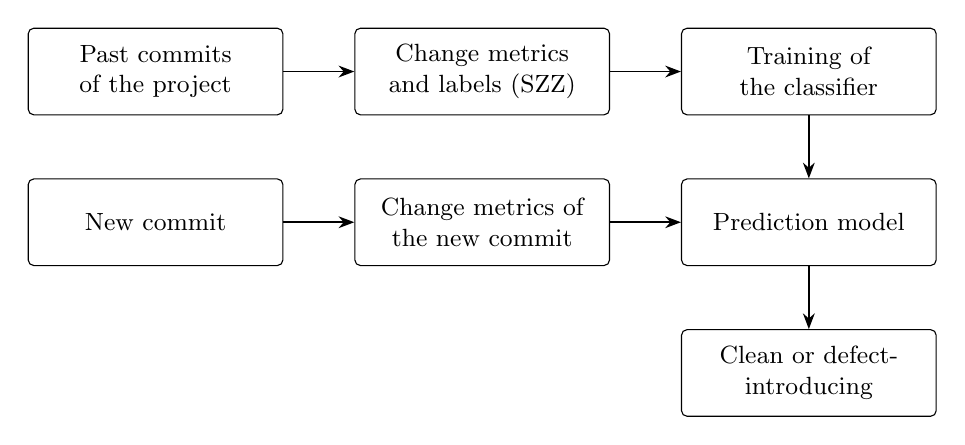
\begin{tikzpicture}[node distance=8mm and 9mm, font=\small,
  box/.style={draw, rounded corners=2pt, align=center, minimum height=11mm, text width=30mm},
  arr/.style={-{Stealth[length=2mm]}, semithick}]
\begin{scope}[every node/.append style={execute at begin node=\setstretch{1}}]
\node[box] (hist) {Past commits of the project};
\node[box, right=of hist] (feat) {Change metrics and labels (SZZ)};
\node[box, right=of feat] (train) {Training of the classifier};
\node[box, below=of train] (model) {Prediction model};
\node[box, left=of model] (newf) {Change metrics of the new commit};
\node[box, left=of newf] (new) {New commit};
\node[box, below=of model] (out) {Clean or defect-introducing};
\end{scope}
\draw[arr] (hist) -- (feat);
\draw[arr] (feat) -- (train);
\draw[arr] (train) -- (model);
\draw[arr] (new) -- (newf);
\draw[arr] (newf) -- (model);
\draw[arr] (model) -- (out);
\end{tikzpicture}
\caption{General workflow of just-in-time software defect prediction.}
\label{fig:workflow}
\end{figure}

Three characteristics of this task are important for the present work. First,
commits arrive one after another in time, so the data form a stream and the
model is always used on commits that are newer than the ones it was trained
on. Second, only a small fraction of the commits introduce defects. In the
dataset used in this work the fraction is 8.54\%, which means that the data
are highly imbalanced. Third, the label of a commit is not known when the
commit is made. It becomes known only later, when the defect is noticed and
fixed, and for a clean commit it is never confirmed at all.

\section{Labelling of Commits and the SZZ Algorithm}

To train a JIT-SDP model, every past commit needs a label that says whether
it introduced a defect. Software repositories do not store this information.
What can be found in a repository and its issue tracker is the set of commits
that \emph{fixed} defects, because developers normally mention the bug report
in the commit message. The commits that \emph{introduced} the defects have to
be inferred from these bug-fixing commits.

The standard method for this inference is the SZZ algorithm, proposed by
\'{S}liwerski, Zimmermann and Zeller~\cite{sliwerski2005szz}. The algorithm
takes a bug-fixing commit and looks at the lines that were deleted or modified
by it. For each of these lines it uses the annotation facility of the version
control system (\texttt{git blame}) to find the earlier commit in which the
line was last changed. These earlier commits are labelled as
defect-introducing. All commits that are never reached in this way are treated
as clean.

Figure~\ref{fig:szzexample} illustrates the procedure with a small example.
Commit $c_2$ adds a faulty line. The fault is corrected later in the
bug-fixing commit $c_5$. When SZZ traces the corrected line back, it reaches
$c_2$, which is the right answer. However, the developer of $c_5$ has also
edited another line that had nothing to do with the bug, for example to
improve the formatting. This line was last changed in $c_3$, so SZZ labels
$c_3$ as defect-introducing as well, although it is clean.

\begin{figure}[htbp]
\centering
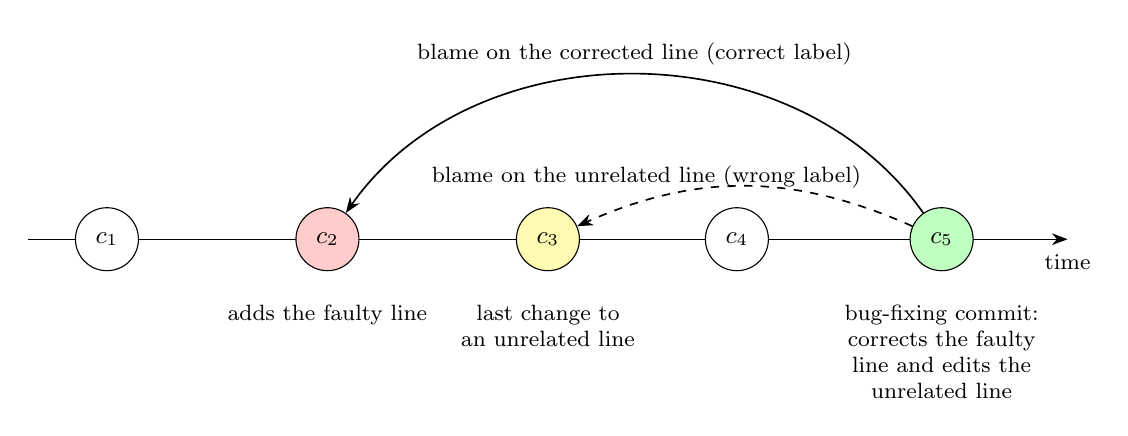
\begin{tikzpicture}[font=\small,
  c/.style={circle, draw, minimum size=8mm, inner sep=0pt},
  note/.style={align=center, font=\footnotesize, text width=27mm}]
\draw[-{Stealth[length=2mm]}] (0,0) -- (13.2,0) node[below=2pt, font=\footnotesize] {time};
\node[c, fill=white] (c1) at (1.0,0) {$c_1$};
\node[c, fill=red!20] (c2) at (3.8,0) {$c_2$};
\node[c, fill=yellow!30] (c3) at (6.6,0) {$c_3$};
\node[c, fill=white] (c4) at (9.0,0) {$c_4$};
\node[c, fill=green!25] (c5) at (11.6,0) {$c_5$};
\begin{scope}[every node/.append style={execute at begin node=\setstretch{1}}]
\node[note, below=3mm of c2] {adds the faulty line};
\node[note, below=3mm of c3] {last change to an unrelated line};
\node[note, below=3mm of c5] {bug-fixing commit: corrects the faulty line and edits the unrelated line};
\end{scope}
\draw[-{Stealth[length=2mm]}, semithick] (c5) to[bend right=55]
   node[above, font=\footnotesize] {blame on the corrected line (correct label)} (c2);
\draw[-{Stealth[length=2mm]}, semithick, dashed] (c5) to[bend right=24]
   node[above=1pt, font=\footnotesize, pos=0.8] {blame on the unrelated line (wrong label)} (c3);
\end{tikzpicture}
\caption{Example of how SZZ identifies defect-introducing commits and how a
change that is unrelated to the fix leads to a wrong label.}
\label{fig:szzexample}
\end{figure}

A bug-fixing commit that contains such unrelated modifications is called a
\emph{tangled} commit. Tangled commits are common. Herbold et
al.~\cite{herbold2022tangling} manually examined a large number of bug-fixing
commits and found that only 17\% to 32\% of the changed lines in them actually
contribute to the bug fix. The remaining lines are changes to tests,
documentation, formatting, refactoring and other modifications. Several
improved versions of SZZ have been proposed to remove such lines before the
blame step, and they are reviewed in Chapter~\ref{ch:lit}. It is important to
note that all of them still \emph{estimate} the label. None of the labels used
in JIT-SDP studies is directly observed.

\section{Motivation}

The motivation for this work comes from four issues in the way JIT-SDP models
are currently built and evaluated.

\paragraph{Noise in the SZZ labels.} Since the labels are produced by a
heuristic, some clean commits are labelled as defect-introducing (false
positives) and some defect-introducing commits are labelled as clean (false
negatives). A model trained on such labels learns partly from wrong examples.
Earlier studies have evaluated the accuracy of SZZ on small manually checked
samples~\cite{dacosta2017maszz,rosa2021oracle}, but the amount and the
type of noise over the complete history of a project, which is what a JIT-SDP
model is trained on, has received less attention.

\paragraph{Evaluation against the same noisy labels.} In nearly all JIT-SDP
studies the test set is labelled by the same SZZ implementation as the
training set. A model is therefore rewarded when it predicts what SZZ would
say, including the cases where SZZ is wrong. The reported performance then
measures how well the model reproduces the labelling heuristic, which is not
the same as how well it finds real defects. The difference between the two can
only be measured if labels from an independent source are available for
testing.

\paragraph{Evaluation that ignores time.} Many studies evaluate their models
with random $k$-fold cross-validation. On commit data this means that the
model may be trained on commits that were made after the commits on which it
is tested. Such a setting cannot occur in practice, and it has been shown for
defect prediction in general that it gives optimistic
results~\cite{falessi2020order,tan2015online}.

\paragraph{Delay in the arrival of labels.} Even when the commits are split
by time, it is normally assumed that the label of every training commit is
known at training time. In reality a defect-introducing commit is recognised
only when its defect is fixed, which may happen months or years later. Cabral
et al.~\cite{cabral2019orb} called this delay \emph{verification latency}.
During the delay the commit is treated as clean, so a model that is updated
continuously receives a wrong label first and the correct label later. In the
dataset used here the median delay is 113 days, and more than half of the
defect labels arrive later than 90 days after the commit.

These four issues are related. The first one is about the quality of the
training data, and the other three are about the realism of the evaluation.
A study that wants to know how much the label noise matters in practice has to
control all of them at the same time.

\section{Problem Statement}

JIT-SDP models are trained and evaluated on labels generated by the SZZ
algorithm, and the evaluation is often carried out without respecting the
order of commits and the delay with which labels become available. As a
result, it is not known how much the errors made by SZZ reduce the ability of
a model to identify real defect-introducing commits when the model is used in
a realistic setting, and it is not possible to say how much of the performance
reported in the literature is due to the model and how much is due to the way
it was evaluated.

The problem addressed in this thesis is therefore to quantify the label noise
introduced by SZZ and its variants, to measure the effect of this noise on
JIT-SDP models under an evaluation that respects time order and verification
latency, and, in the later part of the thesis, to understand how the noise
affects an online learner and how its effect can be reduced.

\section{Scope of this Report}

The thesis work has been planned in stages. This report covers the first
stage, which has been completed. It consists of two connected studies:

\begin{enumerate}[leftmargin=*]
\item an analysis of the quality of the labels produced by six SZZ variants,
measured against a set of reference labels over the full history of 21
projects, and
\item an analysis of the effect of these labels on three JIT-SDP models, which
are evaluated under four evaluation settings of increasing realism and are
scored against the reference labels as well as against their own training
labels.
\end{enumerate}

The questions of how the noise damages an online learner and how a learner
can be made less sensitive to it belong to the next stage of the thesis. They
are described as planned work in Chapter~\ref{ch:conclusion}, and no results
are reported for them here.

\section{Contributions of the First Stage}

The main outcomes of the work reported here are the following.

\begin{itemize}[leftmargin=*]
\item A measurement of the labelling errors of six SZZ variants on 27,319
commits, using the same set of commits for every variant. The errors are
described separately for false positives and false negatives, for the whole
dataset and for each project.
\item An analysis of the agreement between the variants, which shows that
agreement among SZZ variants cannot be taken as evidence that their labels are
correct.
\item A controlled comparison of three prediction models, seven label sets
and four evaluation settings, which separates the effect of the label source
from the effect of the evaluation procedure.
\item An estimate of the loss in prediction performance caused by SZZ labels
when an online learner is evaluated on a commit stream with delayed labels.
\item A reproducible experimental pipeline in which every reported number is
generated by a script from the stored data.
\end{itemize}

\section{Organisation of the Report}

The rest of this report is organised as follows. Chapter~\ref{ch:lit} reviews
the related literature. Chapter~\ref{ch:gaps} lists the research gaps
identified from the literature and states the research questions and
objectives of the thesis. Chapter~\ref{ch:data} describes the dataset.
Chapter~\ref{ch:method} explains the methodology, including the generation of
the SZZ labels, the prediction models, the evaluation settings and the
statistical analysis. Chapter~\ref{ch:results} presents and discusses the
results. Chapter~\ref{ch:conclusion} concludes the report, discusses the
threats to validity and outlines the work planned for the next stage.

% ============================================================================
\chapter{Literature Review}\label{ch:lit}
% ============================================================================

This chapter reviews the literature related to the present work. It starts
with defect prediction in general and JIT-SDP in particular, then discusses
the SZZ algorithm and its variants, the studies on label noise, the evaluation
of prediction models, online learning for imbalanced data streams and learning
with noisy labels. A summary of the most closely related studies is given at
the end of the chapter.

\section{Software Defect Prediction}

Software defect prediction has been studied for more than three decades. The
usual approach is to describe each software module by a set of metrics, such
as size, complexity, coupling or the history of past changes, and to train a
classifier that separates defective modules from clean ones. Hall et
al.~\cite{hall2012slr} carried out a systematic review of 208 fault prediction
studies and observed that models based on simple techniques such as Na\"ive
Bayes and logistic regression often perform as well as more complex ones, and
that the quality of the data and of the experimental procedure has a large
influence on the reported results. Rathore and Kumar~\cite{rathore2019study}
reviewed the field with respect to three aspects: the software metrics used,
the prediction techniques and the data quality issues. Among the data quality
issues they discuss class imbalance and noise in the data, both of which are
central to the present work.

Most of this research predicts defects for files, classes or modules of a
given release. The limitations of this granularity, mentioned in
Chapter~\ref{ch:intro}, led to the prediction of defects at the level of
individual changes.

\section{Just-in-Time Software Defect Prediction}

\subsection{Change-level prediction and change metrics}

Mockus and Weiss~\cite{mockus2000risk} were among the first to predict the
risk of a software change. They used properties of the change, such as its
size, the number of files and subsystems it touches, the experience of the
developer and the type of the change, to predict the probability that a change
to a large telecommunication system would cause a failure. Kim et
al.~\cite{kim2008classifying} introduced \emph{change classification}, in
which a classifier is trained to decide whether a change is buggy or clean.
They used features extracted from the change log, the source code and the
change metadata, and obtained on average 78\% accuracy and 60\% recall for
buggy changes on twelve open-source projects.

Kamei et al.~\cite{kamei2013jit} carried out a large empirical study on six
open-source and five commercial projects and introduced the term
``just-in-time'' for this kind of quality assurance. They proposed fourteen
change metrics that are grouped into five dimensions: diffusion, size,
purpose, history and experience. Their logistic regression model predicted
defect-inducing changes with an average accuracy of 68\% and a recall of 64\%.
These fourteen metrics have become the standard feature set for JIT-SDP and
are also used in the present work. They are described in detail in
Section~\ref{sec:features}. A recent survey by Zhao et
al.~\cite{zhao2023survey} covers 67 JIT-SDP studies and shows that the
majority of them follow the formulation of Kamei et al.\ with respect to both
the features and the way the labels are obtained.

McIntosh and Kamei~\cite{mcintosh2018moving} studied how JIT-SDP models
behave over time on the Qt and OpenStack projects. They found that the
properties of defect-inducing changes are not stable. The importance of the
different metrics changes as a project evolves, and a model loses a
considerable part of its predictive power when it is used long after it was
trained. This result shows that time has to be taken into account both in
training and in evaluating such models.

\subsection{Learning techniques}

A wide range of learning techniques has been applied to JIT-SDP. Besides
logistic regression, random forests and other ensemble methods are frequently
used. More recently, deep learning models have been proposed that learn
features directly from the content of a change. DeepJIT~\cite{hoang2019deepjit}
applies convolutional networks to the commit message and to the changed code.
CC2Vec~\cite{hoang2020cc2vec} learns a vector representation of a code change
with a hierarchical attention network and combines it with DeepJIT.

Later studies have questioned whether this additional complexity is
necessary. Zeng et al.~\cite{zeng2021lapredict} replicated DeepJIT and CC2Vec
on a larger dataset of more than 310,000 changes. They reported that the deep
models did not consistently perform better than traditional approaches, and
that a logistic regression model using only the number of added lines, which
they called LApredict, outperformed both of them in most cases while being
many times faster. Pornprasit and
Tantithamthavorn~\cite{pornprasit2021jitline} proposed JITLine, which uses a
random forest together with oversampling of the minority class, and showed
that it is more accurate and much faster than the deep models. Yang et
al.~\cite{yang2016effort} had earlier shown for effort-aware prediction that
simple unsupervised models built from a single change metric can be better
than supervised models.

These studies are relevant here for two reasons. First, they show that the
ranking of models in JIT-SDP depends strongly on how the evaluation is done.
Second, they provide two well-known models of very different complexity,
LApredict and JITLine, which are used in the present work to examine whether
the effect of label noise depends on the capacity of the model.

\section{Identification of Defect-Introducing Changes}

\subsection{The SZZ algorithm}

The SZZ algorithm~\cite{sliwerski2005szz} consists of two phases. In the
first phase, bug-fixing commits are identified by linking the commits of the
version control system to the reports in the bug tracking system, mainly by
searching the commit messages for bug identifiers. In the second phase, for
every bug-fixing commit the lines that were deleted or modified are
determined, and the annotate (blame) command is used to find the most recent
earlier commits that changed these lines. Commits that were made after the bug
was reported are excluded, since they cannot have caused the bug. The
remaining commits are considered to be bug-introducing.

The algorithm depends on two assumptions. The first is that the lines changed
by the fix are the lines that contained the defect. The second is that the
commit that last changed such a line is the commit that made it defective.
Both assumptions can fail. The first one fails for tangled commits, where
some of the changed lines are not related to the fix. The second one fails
when a line was last touched by a cosmetic change, such as a renaming or
re-indentation, so that the blame points to this change instead of the
original faulty one. In addition, a defect that is fixed only by adding new
lines leaves no deleted or modified line to trace, and a defect caused by a
change in the environment or in the requirements has no introducing commit in
the repository at all~\cite{rodriguez2020bugs}.

\subsection{Variants of SZZ}

Several variants have been proposed to reduce the number of wrong labels
produced by the original algorithm, which is usually called B-SZZ (basic
SZZ). Table~\ref{tab:variants} lists the variants that are studied in this
work.

\begin{table}[htbp]
\centering\small
\caption{SZZ variants considered in this work.}
\label{tab:variants}
\begin{tabularx}{\linewidth}{@{}l>{\raggedright\arraybackslash}X@{}}
\toprule
Variant & Main idea \\
\midrule
B-SZZ~\cite{sliwerski2005szz} & Original algorithm. Every line deleted or
modified by the bug-fixing commit is traced back with blame. \\
AG-SZZ~\cite{kim2006agszz} & Uses an annotation graph to follow lines across
revisions and ignores blank lines, comments and formatting changes. \\
MA-SZZ~\cite{dacosta2017maszz} & Builds on AG-SZZ and additionally ignores
meta-changes, i.e.\ branch changes, merge changes and property changes, which
do not modify the source code. \\
R-SZZ~\cite{davies2014rlszz} & Builds on MA-SZZ and keeps, for each bug-fixing
commit, only the most recent of the candidate commits. \\
L-SZZ~\cite{davies2014rlszz} & Builds on MA-SZZ and keeps only the candidate
commit that changed the largest number of lines. \\
RA-SZZ~\cite{neto2018raszz} & Builds on MA-SZZ and ignores lines that were
changed by refactoring operations, which are detected with a refactoring
detection tool. It is available for Java only. \\
\bottomrule
\end{tabularx}
\end{table}

Kim et al.~\cite{kim2006agszz} observed that many lines changed in a
bug-fixing commit are comments, blank lines or formatting changes and proposed
to ignore them. They also replaced the simple annotate command by an
annotation graph, which follows a line more reliably when code is moved. Da
Costa et al.~\cite{dacosta2017maszz} noticed that some commits flagged by SZZ
are only changes to the repository structure, such as merges, and excluded
these meta-changes. R-SZZ and L-SZZ go one step further and select a single
commit from the candidates returned for a bug-fixing
commit~\cite{davies2014rlszz}. They assume that a bug has one introducing
commit and choose either the latest or the largest candidate. Neto et
al.~\cite{neto2018raszz} showed that refactoring operations are a frequent
cause of wrong labels and proposed RA-SZZ, which removes refactored lines
from the analysis.

All these variants try to reduce false positives by removing lines or
candidate commits. An obvious consequence, which is examined in
Chapter~\ref{ch:results}, is that some correct candidates may be removed as
well.

\subsection{Empirical evaluations of SZZ}

The accuracy of SZZ is difficult to evaluate, because the true
defect-introducing commits are not known. Da Costa et
al.~\cite{dacosta2017maszz} proposed a framework that evaluates SZZ
implementations indirectly through three criteria: the earliest appearance of
the bug, the future impact of the flagged changes and the realism of the bug
introduction. They applied it to five implementations on ten open-source
projects and found that the existing implementations still have considerable
room for improvement.

Rodr\'{\i}guez-P\'{e}rez et al.~\cite{rodriguez2018szz} reviewed 187 papers
that use SZZ and found that most of them neither discuss the limitations of
the algorithm nor provide enough detail to reproduce the labelling. In a later
study~\cite{rodriguez2020bugs} they manually analysed how 116 bugs were
introduced in two open-source projects. They found that a part of the bugs
are \emph{extrinsic}, i.e.\ caused by changes outside the project code, and
that the SZZ-based algorithms reached F-scores of only 0.44 to 0.77 on the
remaining ones.

Rosa et al.~\cite{rosa2021oracle,rosa2023szzvariants} built a
\emph{developer-informed oracle} from commit messages in which the developer
explicitly names the commit that introduced the bug being fixed. The oracle
contains 1,930 such cases, extended to 2,304 in the journal version, and was
used to compare several SZZ variants. R-SZZ obtained the best results, with a
precision of about 66\% and an F-measure of about 61\%, while B-SZZ had a
higher recall but a precision of only about 39\%. The authors also released
PySZZ, an open-source implementation of the variants, which is used in the
present work.

Two properties of this oracle are important for the present study. It
contains only bug-fixing commits together with their introducing commits and
no clean commits, so it cannot be used to train or test a JIT-SDP model. It
also evaluates SZZ only on fixes for which an introducing commit is known to
exist. This is a different question from the one that matters for JIT-SDP,
where every commit in the history of the project receives a label.

\subsection{Tangled changes}

Herzig and Zeller~\cite{herzig2013tangled} studied tangled changes in five
open-source Java projects and found that up to 15\% of the bug fixes consist
of several unrelated changes. As a result, at least 16.6\% of the source files
were incorrectly associated with bug reports. Herbold et
al.~\cite{herbold2022tangling} conducted a large crowd-sourced study in which
every changed line of the bug-fixing commits of several Apache projects was
labelled by four participants. They found that only 17\% to 32\% of all
changed lines contribute to the bug fix. When only changes to production code
files are considered, the share is 66\% to 87\%. For about 11\% of the lines
the participants could not agree on a label. The dataset produced by this
study, called LLTC4J, is the basis of the reference labels used in the present
work (Section~\ref{sec:reference}).

\section{Label Noise in Defect Prediction}

The effect of wrong labels on defect prediction models has been studied
mainly for file-level prediction. Kim et al.~\cite{kim2011noise} added
artificial false positive and false negative noise to defect datasets and
found that the prediction performance decreases significantly once the
datasets contain about 20\% to 35\% of both types of noise. They also proposed
a method to detect and remove noisy instances. Tantithamthavorn et
al.~\cite{tantithamthavorn2015mislabelling} examined mislabelling that arises
from wrongly classified issue reports. They showed that such mislabelling is
not random, and that models trained on the noisy data keep their precision
but reach only 56\% to 68\% of the recall of models trained on clean data.

For JIT-SDP, the most closely related study is that of Fan et
al.~\cite{fan2021mislabeled}. They labelled 126,526 changes from ten Apache
projects with four SZZ variants (B-SZZ, AG-SZZ, MA-SZZ and RA-SZZ) and
examined how the differences between the variants affect JIT-SDP models. They
reported that the changes mislabelled by B-SZZ and MA-SZZ do not reduce the
prediction performance considerably, whereas those mislabelled by AG-SZZ lead
to a statistically significant reduction. Since no ground truth was available,
they treated the labels of RA-SZZ as correct and measured the mislabelling of
the other variants relative to it. This has two consequences. The noise of
RA-SZZ itself could not be measured, and errors that are common to all
variants, for example those caused by tangled changes, remained invisible. The
study also did not consider the delayed arrival of labels.

\section{Evaluation of Defect Prediction Models}

\subsection{Validation schemes and time order}

Cross-validation with random folds is the most common validation scheme in
defect prediction. For data that are ordered in time it has a known weakness,
because a model can be trained on data that are newer than the test data. Tan
et al.~\cite{tan2015online} pointed out for change classification that
cross-validation uses information from the future and can therefore report a
precision that is too high. They proposed a time-sensitive evaluation in
which the model is trained only on changes that precede the test changes.
Falessi et al.~\cite{falessi2020order} analysed this issue systematically for
within-project defect classifiers. They showed that validation techniques
which do not preserve the order of the data produce results that differ from
those of order-preserving techniques, and recommended the latter. In spite of
these findings, random cross-validation is still widely used in JIT-SDP
studies~\cite{zhao2023survey}.

\subsection{Prequential evaluation}

When data arrive as a stream, the standard evaluation procedure is
\emph{prequential} (predictive sequential) evaluation, also known as
test-then-train. Each example is first used to test the model and afterwards
to update it. The performance is accumulated over the stream. Since the
performance at the beginning of the stream is often poor and less relevant, a
forgetting mechanism such as a sliding window or a fading factor is applied.
Gama et al.~\cite{gama2013prequential} showed that the prequential error
computed with a fading factor converges to the same value as the error on an
independent holdout set. This result holds for the error rate. For measures
that are computed from the complete confusion matrix, such as MCC, no
corresponding result is available, which has to be kept in mind when
prequential values of such measures are summarised
(Section~\ref{sec:measures}).

\subsection{Verification latency}

Cabral et al.~\cite{cabral2019orb} were the first to investigate JIT-SDP as an
online learning problem with verification latency. In their setting a commit
is used as a clean training example when a waiting period has passed without
a defect being linked to it, and as a defect-inducing example as soon as a
defect is linked to it. They used a waiting period of 90 days. They showed
that, because of this mechanism, the proportion of the two classes seen by
the learner changes over time, which they called class imbalance evolution,
and that this hinders the existing approaches. To deal with it they proposed
the ORB method, which is described in Section~\ref{sec:lit-online}. In a later
study, Cabral and Minku~\cite{cabral2023reliable} examined concept drift in
JIT-SDP in more detail. They reported that the time needed to discover a
defect ranges from one day to more than eleven years, and proposed a method
that also uses the predictions on unlabelled commits to detect when the model
has become unreliable. Tabassum et al.~\cite{tabassum2020cross} studied the
use of data from other projects in the same online setting.

In these studies the wrong labels that the learner receives are caused by
time: a defect-introducing commit is treated as clean until its defect is
found. The labels that finally arrive are assumed to be correct. The noise
that comes from the SZZ algorithm itself, where the final label is wrong and
is never corrected, is not addressed.

\subsection{Performance measures}

Because the classes are imbalanced, accuracy is not a suitable measure for
defect prediction. Precision, recall and the F-measure are widely used, but
the F-measure ignores the true negatives and depends on the proportion of the
positive class. Yao and Shepperd~\cite{yao2020mcc} showed that the use of the
F-measure can lead to different conclusions than the Matthews correlation
coefficient (MCC)~\cite{matthews1975mcc} in a considerable number of defect
prediction comparisons and recommended MCC. Chicco and
Jurman~\cite{chicco2020mcc} reached the same recommendation for binary
classification in general. MCC uses all four cells of the confusion matrix
and takes the value zero for a classifier that predicts at random or always
predicts the same class. For measuring the agreement between two sets of
labels, Cohen's $\kappa$~\cite{cohen1960kappa} is commonly used, which
corrects the observed agreement for the agreement expected by chance. Landis
and Koch~\cite{landis1977kappa} proposed the widely used verbal
interpretation of $\kappa$ values, according to which values up to 0.20
indicate slight agreement and values above 0.80 almost perfect agreement.

\section{Online Learning for Imbalanced Data Streams}\label{sec:lit-online}

Online Bagging~\cite{oza2001onlinebagging} is the online version of the
bagging ensemble. In ordinary bagging each base learner is trained on a
bootstrap sample of the data. In the online version, each arriving example is
presented to each base learner $k$ times, where $k$ is drawn from a Poisson
distribution with parameter $\lambda = 1$. Wang et al.~\cite{wang2015oob}
adapted this method to imbalanced streams. In their Oversampling Online
Bagging (OOB), the parameter $\lambda$ for an example of the minority class
is increased according to the current ratio of the class sizes, so that
minority examples are presented more often. The class sizes are tracked with
a time-decayed average, which allows the method to follow changes in the
imbalance.

ORB (Oversampling Rate Boosting)~\cite{cabral2019orb} extends OOB for
JIT-SDP. It monitors the predictions that the model has made recently. If the
model predicts one class much more often than expected, the resampling rate
of the other class is increased further by a boosting factor. In this way the
model is pushed back when it becomes biased towards one class, which happens
frequently under verification latency.

It should be noted that in all these methods the resampling rate depends only
on how many examples of each class have been observed. Whether the labels of
these examples are correct plays no role. A commit that is wrongly labelled
as defect-introducing is oversampled in the same way as a correctly labelled
one. This property is one of the reasons why the effect of label noise on
such learners deserves to be studied.

\section{Learning with Noisy Labels}

In the machine learning literature, several methods have been proposed for
training classifiers on data with wrong labels. Natarajan et
al.~\cite{natarajan2013noisy} considered the case where the probability that
a label is flipped depends on the class, which is called class-conditional
noise. They showed that, if the two flip rates are known, the loss function
can be modified such that minimising it on the noisy data is equivalent in
expectation to minimising the original loss on clean data. The correction
contains the factor $1/(1-\rhoz-\rhoo)$, where $\rhoz$ and $\rhoo$ are the
two flip rates, and becomes unstable when the sum of the rates approaches
one. Co-teaching~\cite{han2018coteaching} trains two neural networks at the
same time. Each network selects the examples with small loss in a mini-batch,
which are likely to be correctly labelled, and passes them to the other
network for training. Confident learning~\cite{northcutt2021confident}
estimates the joint distribution of the given and the true labels from the
predicted probabilities of a classifier and uses it to identify and remove
the examples that are probably mislabelled.

These methods were developed for the batch setting, in which the complete
dataset is available and can be processed several times. They also assume
that a wrong label stays wrong. In online JIT-SDP each example is seen once,
its label arrives late, and a label may be changed later from clean to
defect-introducing. The methods can therefore not be applied directly, but
the class-conditional noise model on which they are based is the one that is
measured in the present work.

\section{Summary}

Table~\ref{tab:litsummary} summarises the studies that are most closely
related to the present work and indicates in which respect each of them
differs from it. The review shows that the accuracy of SZZ, the effect of
label noise, time-aware evaluation and verification latency have each been
studied, but mostly in isolation. The gaps that follow from this are stated
in the next chapter.

\begin{table}[htbp]
\centering\footnotesize
\setlength{\tabcolsep}{4pt}
\caption{Summary of the most closely related studies.}
\label{tab:litsummary}
\begin{tabularx}{\linewidth}{@{}>{\raggedright\arraybackslash}p{27mm}>{\raggedright\arraybackslash}p{40mm}>{\raggedright\arraybackslash}X@{}}
\toprule
Study & Focus & Difference from the present work \\
\midrule
Kamei et al.~\cite{kamei2013jit} & Change metrics and models for JIT-SDP &
Labels from SZZ are taken as correct; no time-aware evaluation \\
Da Costa et al.~\cite{dacosta2017maszz} & Framework for evaluating SZZ
implementations & Indirect criteria; effect on prediction models not studied \\
Rosa et al.~\cite{rosa2021oracle,rosa2023szzvariants} & Accuracy of SZZ
variants against a developer-informed oracle & Oracle has no clean commits;
effect on prediction models not studied \\
Herbold et al.~\cite{herbold2022tangling} & Amount of tangling in bug-fixing
commits & Line-level analysis; labels of commits and models not studied \\
Kim et al.~\cite{kim2011noise} & Artificial label noise in file-level defect
data & Noise is injected artificially; file-level prediction with batch evaluation \\
Fan et al.~\cite{fan2021mislabeled} & Effect of labels of four SZZ variants on
JIT-SDP & RA-SZZ used as reference; no independent labels; no latency \\
Falessi et al.~\cite{falessi2020order} & Order-preserving validation of defect
classifiers & Label noise not considered \\
Cabral et al.~\cite{cabral2019orb} & Online JIT-SDP with verification latency
and class imbalance evolution & SZZ labels taken as correct once they arrive \\
Zeng et al.~\cite{zeng2021lapredict} & Comparison of deep and simple JIT-SDP
models & Label noise and latency not considered \\
Natarajan et al.~\cite{natarajan2013noisy} & Learning under class-conditional
label noise & Batch setting; noise rates assumed to be known \\
\bottomrule
\end{tabularx}
\end{table}

% ============================================================================
\chapter{Research Gaps, Research Questions and Objectives}\label{ch:gaps}
% ============================================================================

This chapter states the research gaps that were identified from the
literature reviewed in Chapter~\ref{ch:lit}. Based on these gaps, the research
questions and the objectives of the thesis are formulated. The part of the
objectives that is covered by the first stage of the work is indicated.

\section{Research Gaps}

The following gaps were identified.

\paragraph{Gap 1: The noise of SZZ labels has not been measured over complete
project histories.} The existing evaluations of SZZ either use indirect
criteria~\cite{dacosta2017maszz} or check the algorithm on a sample of
bug-fixing commits for which the introducing commit is
known~\cite{rosa2021oracle,rodriguez2020bugs}. These evaluations tell how
often SZZ finds the right commit for a given fix. They do not tell how many
of the commits in the history of a project receive a wrong label, which is
the quantity that matters for a JIT-SDP model, because the model is trained on
all commits. In particular, the rate of false positives among the clean
commits and the rate of false negatives among the defect-introducing commits
have not been reported separately for the different variants.

\paragraph{Gap 2: Models are tested against the same labels on which they are
trained.} In the JIT-SDP literature the test labels come from the same SZZ
implementation as the training labels. The study that is closest to the
present work~\cite{fan2021mislabeled} used one SZZ variant as the reference
for the others. Hence it is not known how well a model that was trained on
SZZ labels predicts labels that were obtained independently of the SZZ
variant used for training.

\paragraph{Gap 3: The effect of label noise has not been separated from the effect
of the evaluation procedure.} It is known that random cross-validation gives
optimistic results for time-ordered
data~\cite{falessi2020order,tan2015online}, and it is known that SZZ labels
contain errors. These two factors are present together in most published
results, and their individual contributions have not been measured in a
common experimental design.

\paragraph{Gap 4: Label noise has not been studied under verification latency.}
The studies on online JIT-SDP~\cite{cabral2019orb,cabral2023reliable} model
the delay of the labels but assume that the labels which finally arrive are
correct. The studies on label noise use batch
evaluation~\cite{kim2011noise,fan2021mislabeled}. The loss caused by SZZ
noise for an online learner that receives delayed labels is therefore not
known.

\paragraph{Gap 5: The way in which SZZ noise affects an online learner is not
understood, and no remedy designed for this setting exists.} Online learners
for imbalanced streams oversample the minority class according to the number
of positive labels they observe (Section~\ref{sec:lit-online}), without
regard to their correctness. Whether false positives or false negatives are
more harmful for such learners is not known. The existing methods for
learning with noisy labels assume a batch setting and stable
labels~\cite{natarajan2013noisy,northcutt2021confident} and cannot be applied
directly to a stream with delayed labels.

\section{Research Questions}

Based on these gaps, the thesis addresses the following research questions.

\paragraph{RQ1: How much do the labels of different SZZ variants disagree with one
another and with independently obtained reference labels, and what type of
error does each variant make?}
This question corresponds to Gap~1. To answer it, the labels of six SZZ
variants are compared with reference labels on the same set of commits, and
the false positive and false negative rates of each variant are estimated.

\paragraph{RQ2: How does the choice of the label source affect the measured
performance of JIT-SDP models under different evaluation settings?}
This question corresponds to Gaps~2, 3 and~4. To answer it, models are
trained on the reference labels and on the labels of each SZZ variant, and
are evaluated with random cross-validation, with a chronological split and
with prequential evaluation under verification latency. The predictions are
scored against the reference labels and, for comparison, against the training
labels.

\paragraph{RQ3: Through which mechanism does label noise reduce the performance of
an online learner, and which of the two types of error is responsible?}
This question corresponds to the first part of Gap~5. It will be addressed in
the next stage of the thesis.

\paragraph{RQ4: Can an online learner be modified so that it loses less
performance when it is trained on SZZ labels, without access to clean labels
and without losing performance when the labels are clean?}
This question corresponds to the second part of Gap~5. It will also be
addressed in the next stage of the thesis.

\section{Objectives}

The objectives of the thesis are as follows.

\begin{enumerate}[leftmargin=*]
\item To generate the labels of six SZZ variants for all projects of a
dataset that provides independent reference labels, and to characterise the
labelling errors of each variant in terms of false positive and false
negative rates.
\item To examine the agreement between the SZZ variants and to identify the
sources of the errors that the variants make.
\item To measure how much the evaluation procedure, namely the validation
scheme and the labels used for scoring, changes the measured performance of
JIT-SDP models.
\item To measure the loss in performance caused by training on SZZ labels
when an online learner is evaluated on a commit stream with verification
latency.
\item To identify the type of labelling error that is responsible for this
loss and the mechanism through which it acts.
\item To design and evaluate a modification of the online learner that
reduces this loss.
\end{enumerate}

Objectives 1 to 4 belong to the first stage of the thesis and have been
completed. They are reported in the following chapters. Objectives 5 and 6
belong to the next stage, and the plan for them is given in
Section~\ref{sec:future}.

\section{Scope of the First Stage}

The work reported here is limited in the following ways. It uses one dataset
of 21 Java projects, because independent reference labels at the level of
commits are available only for this dataset. It uses the fourteen change
metrics of Kamei et al.\ as features and does not consider features derived
from the source code or the commit message. Three models are studied, which
were selected to cover a simple batch model, a more complex batch model and
an online model. The analysis is exploratory in the sense that the
comparisons to be made were not fixed before the data were examined. For this
reason a correction for multiple comparisons is applied to all tests together
(Section~\ref{sec:stats}).

% ============================================================================
\chapter{Dataset}\label{ch:data}
% ============================================================================

This chapter describes the dataset used in the study. It first states the
requirements that the dataset has to satisfy and then describes the
JIT-Defects4J dataset, the projects it contains, the reference labels, the
change metrics and the data on the arrival time of the labels.

\section{Requirements}

The research questions place several requirements on the dataset.

\begin{itemize}[leftmargin=*]
\item A label must be available for every commit of a project, including the
clean commits, because JIT-SDP models are trained and tested on the complete
commit history.
\item The labels must not have been produced by the SZZ variant that is being
evaluated. Otherwise the errors of that variant cannot be observed.
\item The change metrics of the commits must be available, so that prediction
models can be trained.
\item The repositories of the projects must be accessible, because the SZZ
variants have to be executed on them and the dates of the bug-fixing commits
are needed for simulating verification latency.
\item The dataset should contain several projects, so that the comparisons
can be tested statistically across projects.
\end{itemize}

Most JIT-SDP datasets do not satisfy the second requirement.
ApacheJIT~\cite{keshavarz2022apachejit}, which contains 106,674 commits, and
Defectors~\cite{mahbub2023defectors} are much larger than the dataset used
here, but their labels were generated with SZZ. The developer-informed oracle
of Rosa et al.~\cite{rosa2021oracle} does not satisfy the first requirement,
since it contains no clean commits. The JIT-Defects4J dataset satisfies all
five requirements and was therefore selected.

\section{The JIT-Defects4J Dataset}

JIT-Defects4J was published by Ni et al.~\cite{ni2022jitdefects4j} together
with their JIT-Fine approach. It was built from LLTC4J, the dataset of Herbold
et al.~\cite{herbold2022tangling}, in which the changed lines of bug-fixing
commits were labelled manually. JIT-Defects4J contains 27,319 commits from 21
open-source Java projects of the Apache Software Foundation. For every commit
it provides the fourteen change metrics of Kamei et al.\ and a label that
indicates whether the commit introduced a defect. The dataset was used as it
was published. No project was added or removed, so the selection of projects
could not be influenced by the results of this study.

\section{Subject Projects}

Table~\ref{tab:projects} lists the 21 projects. Sixteen of them are libraries
of the Apache Commons family. The other five are a dependency manager
(ant-ivy), a graph processing system (giraph), a data persistence framework
(gora), a natural language processing toolkit (opennlp) and a columnar storage
format (parquet-mr). The commits were made between 2001 and 2019. The length
of the covered history of a project varies from about 6 years (parquet-mr) to
about 18 years (commons-dbcp).

\begin{table}[htbp]
\centering\small
\caption{Projects of the JIT-Defects4J dataset. The last two columns give the
number and the percentage of defect-introducing commits according to the
reference labels.}
\label{tab:projects}
\begin{tabular}{@{}lcrrrr@{}}
\toprule
Project & Period & Commits & Bug-fixing & \multicolumn{2}{c}{Defect-introducing} \\
\cmidrule(l){5-6}
 & & & commits & Number & \% \\
\midrule
ant-ivy & 2005--2018 & 1,771 & 761 & 332 & 18.7 \\
commons-bcel & 2001--2019 & 825 & 134 & 60 & 7.3 \\
commons-beanutils & 2001--2018 & 611 & 197 & 37 & 6.1 \\
commons-codec & 2003--2018 & 761 & 122 & 36 & 4.7 \\
commons-collections & 2001--2018 & 1,823 & 360 & 50 & 2.7 \\
commons-compress & 2003--2018 & 1,630 & 175 & 178 & 10.9 \\
commons-configuration & 2003--2018 & 1,838 & 358 & 155 & 8.4 \\
commons-dbcp & 2001--2019 & 1,037 & 348 & 58 & 5.6 \\
commons-digester & 2001--2017 & 1,079 & 221 & 19 & 1.8 \\
commons-io & 2002--2018 & 1,142 & 224 & 73 & 6.4 \\
commons-jcs & 2002--2018 & 831 & 237 & 88 & 10.6 \\
commons-lang & 2002--2018 & 2,969 & 491 & 146 & 4.9 \\
commons-math & 2003--2018 & 4,026 & 758 & 335 & 8.3 \\
commons-net & 2002--2018 & 1,121 & 197 & 117 & 10.4 \\
commons-scxml & 2005--2018 & 544 & 55 & 47 & 8.6 \\
commons-validator & 2002--2018 & 598 & 120 & 36 & 6.0 \\
commons-vfs & 2002--2018 & 1,110 & 201 & 114 & 10.3 \\
giraph & 2010--2018 & 844 & 118 & 163 & 19.3 \\
gora & 2010--2019 & 553 & 85 & 39 & 7.1 \\
opennlp & 2010--2018 & 1,086 & 83 & 91 & 8.4 \\
parquet-mr & 2012--2018 & 1,120 & 208 & 158 & 14.1 \\
\midrule
Total & & 27,319 & 5,453 & 2,332 & 8.54 \\
\bottomrule
\end{tabular}
\end{table}

In total, 5,453 commits (20.0\%) are marked as bug-fixing and 2,332 commits
(8.54\%) are defect-introducing according to the reference labels. The
projects differ considerably in size and in the proportion of
defect-introducing commits, as can be seen in Figure~\ref{fig:projects}. The
smallest project has 544 commits and the largest has 4,026. The number of
defect-introducing commits ranges from 19 in commons-digester to 335 in
commons-math, and the defect rate ranges from 1.8\% to 19.3\%. In every
project the defect-introducing commits are a clear minority. Because of these
differences, all comparisons in this work are made project by project and the
results are then summarised over the projects (Section~\ref{sec:stats}).

\begin{figure}[htbp]
\centering
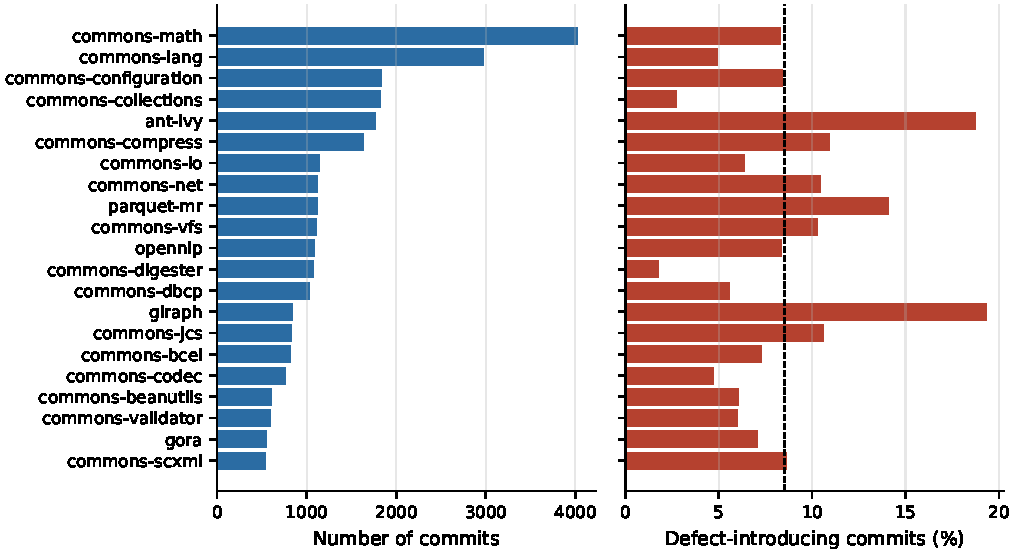
\includegraphics[width=0.95\linewidth]{fig_projects}
\caption{Number of commits and percentage of defect-introducing commits in
each project. The dashed line marks the percentage in the whole dataset
(8.54\%).}
\label{fig:projects}
\end{figure}

\section{Reference Labels}\label{sec:reference}

The label provided with JIT-Defects4J is used in this work as the reference
against which the SZZ variants and the predictions of the models are
assessed. Since all later results depend on this label, its construction is
described in detail.

According to the description given by the authors of the
dataset~\cite{ni2022jitdefects4j}, the labels were obtained in two steps. In
the first step, they took the bug-fixing commits of LLTC4J. In LLTC4J every
changed line of a bug-fixing commit was labelled by four participants, and a
line is regarded as contributing to the bug fix only if at least three of
them assigned this label. In the second step, \texttt{git blame} was applied
to each of these validated lines to find the commit that introduced it. The
commits found in this way are the defect-introducing commits. All other
commits are considered clean.

To make sure that the labels in the files used for the experiments are indeed
these labels, the number of commits and of defect-introducing commits of
every project was compared with the numbers reported in the paper. They agree
for all 21 projects.

The reference labels are thus the result of the blame operation applied to
manually validated bug-fixing lines. They are not a manual judgement about
each commit. This has the following consequences for the interpretation of
the results.

\begin{enumerate}[leftmargin=*]
\item The reference labels and the SZZ labels differ in the lines from which
the tracing starts. SZZ starts from all lines changed in a bug-fixing commit
(after the filtering applied by the particular variant), whereas the reference
starts only from the lines that were confirmed to be part of the fix. A
comparison between the two therefore shows the effect of tangled changes, and
of the filters that the variants use to deal with them.
\item Both use the blame operation to go from a line to a commit. Errors of
the blame operation itself, for example when a line was last touched by a
cosmetic change, are present in both and cannot be detected by comparing
them. The amount of noise measured in this work should therefore be regarded
as a lower bound of the true amount.
\item Every commit that is defect-introducing according to the reference can
be reached by blame from some line of a bug-fixing commit. When an SZZ
variant misses such a commit, the reason cannot be that blame is unable to
reach it. The reason must lie in the lines selected or in the filtering of the
candidates. This fact is used in Section~\ref{sec:fn-sources}.
\item The authors of the dataset excluded changes that do not add any line.
Defects that are introduced only by deleting code are therefore not
represented.
\end{enumerate}

In the rest of this report the term \emph{reference labels} is used for these
labels. The term ``ground truth'' is avoided, because the labels are more
reliable than SZZ labels with respect to tangling but are not free of error.

\section{Change Metrics}\label{sec:features}

Each commit is described by the fourteen change metrics proposed by Kamei et
al.~\cite{kamei2013jit}. They are listed in Table~\ref{tab:metrics}. The
metrics of the diffusion group measure how widely a change is spread over the
code base, since changes that touch many parts are more difficult to
understand. The size group measures how much code was changed. The purpose
group contains a single metric which indicates whether the change is a bug
fix, since bug fixes are known to introduce new defects more often than other
changes. The history group describes how the modified files were changed in
the past, and the experience group describes how familiar the developer is
with the project and with the modified subsystem.

\begin{table}[htbp]
\centering\small
\caption{The fourteen change metrics used as features~\cite{kamei2013jit}.}
\label{tab:metrics}
\begin{tabularx}{\linewidth}{@{}llX@{}}
\toprule
Group & Metric & Description \\
\midrule
Diffusion & NS & Number of modified subsystems \\
 & ND & Number of modified directories \\
 & NF & Number of modified files \\
 & Entropy & Distribution of the modified code across the files \\
\midrule
Size & LA & Lines of code added \\
 & LD & Lines of code deleted \\
 & LT & Lines of code in the files before the change \\
\midrule
Purpose & FIX & Whether the change is a defect fix \\
\midrule
History & NDEV & Number of developers that changed the modified files \\
 & AGE & Average time interval between the last and the current change \\
 & NUC & Number of unique changes to the modified files \\
\midrule
Experience & EXP & Number of changes made by the developer so far \\
 & REXP & Recent experience of the developer (changes weighted by their age) \\
 & SEXP & Experience of the developer on the modified subsystem \\
\bottomrule
\end{tabularx}
\end{table}

The values of the metrics were taken from the dataset as published and were
not recomputed. In this way the features are identical for all label sources,
and differences between the results obtained with different labels cannot be
caused by differences in feature extraction. Several of the metrics have
strongly skewed distributions. The transformations applied to them are part
of the prediction models and are described in Section~\ref{sec:models}.

\section{Label Sets}

Besides the reference label, six further labels were attached to every
commit, one for each SZZ variant of Table~\ref{tab:variants}. They were
generated in this work by running the variants on the repositories of the 21
projects, as described in Section~\ref{sec:szz-generation}. Each commit of the
dataset therefore has seven binary labels. The data used in the experiments
consist of one record per commit with the project name, the commit
identifier, the author timestamp, the fourteen metrics, the seven labels and
the label arrival times described in Section~\ref{sec:latency-data}.

\section{Data Preparation}

The dataset is distributed in three files that correspond to the training,
validation and test split used by its authors. These files were merged, since
the present work uses its own evaluation settings. Duplicate records were
removed on the combination of project and commit identifier. Within each
project the commits were sorted by their author timestamp. This order defines
the commit stream of the project and is used in all evaluation settings that
depend on time.

The repositories of the 21 projects were cloned from GitHub for two purposes:
to run the SZZ variants and to obtain the dates of the bug-fixing commits.
The outputs of both steps were stored as small derived files, so that the
experiments on the prediction models can be repeated without the repositories.

\section{Label Arrival Times}\label{sec:latency-data}

To evaluate an online learner realistically, it must be known when the label
of each commit would have become available. For a defect-introducing commit
this is the time at which its defect was fixed, because only then the commit
can be identified as the origin of the defect.

The arrival times were obtained as follows. The author date of each of the
5,453 bug-fixing commits was extracted from the repositories. Each SZZ
variant produces a mapping from bug-fixing commits to the commits it
considers defect-introducing. For a commit flagged by a variant, the arrival
time of its label under that variant is the date of the earliest bug-fixing
commit that is mapped to it. The verification latency of the commit is the
difference between this date and the date of the commit itself.

Table~\ref{tab:latency} summarises the latencies over all commits that are
linked to at least one bug-fixing commit, and Figure~\ref{fig:latency} shows
their distribution. The distribution is strongly skewed. About one third of
the labels arrive within 30 days, but the median is 113 days and one tenth
of the labels need more than four years. With the waiting period of 90 days
that is commonly used in online JIT-SDP~\cite{cabral2019orb}, 53.0\% of the
defect labels arrive only after the waiting period has ended. As explained in
Section~\ref{sec:latency-method}, these commits are first presented to the
learner as clean.

\begin{table}[htbp]
\centering\small
\caption{Verification latency of the commits that are linked to a bug-fixing
commit.}
\label{tab:latency}
\begin{tabular}{@{}lr@{}}
\toprule
Statistic & Value \\
\midrule
Commits linked to a bug-fixing commit & 8,819 \\
Lower quartile of the latency & 8 days \\
Median latency & 113 days \\
Upper quartile of the latency & 611 days \\
90th percentile of the latency & 1,597 days \\
Labels arriving within 30 days & 35.2\% \\
Labels arriving after 90 days & 53.0\% \\
Labels arriving after one year & 33.1\% \\
Labels arriving after three years & 16.2\% \\
\bottomrule
\end{tabular}
\end{table}

\begin{figure}[htbp]
\centering
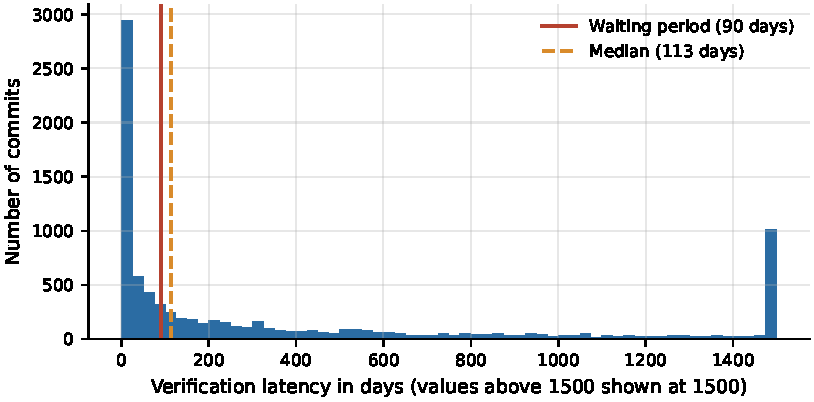
\includegraphics[width=0.85\linewidth]{fig_latency}
\caption{Distribution of the verification latency. A large part of the
labels arrives after the waiting period of 90 days.}
\label{fig:latency}
\end{figure}

The reference labels need a separate treatment. The published dataset
contains the label of each commit but not the link between a
defect-introducing commit and the commit that fixed it. The arrival time of a
reference label was therefore taken from the SZZ mappings: it is the date of
the earliest bug-fixing commit that any of the six variants links to the
commit. For 67.8\% of the 2,332 defect-introducing commits such a link
exists. For the remaining 32.2\% no arrival time is available, and in the
online evaluation their defect label never arrives.

Table~\ref{tab:latency-source} gives the latency separately for each label
source. The medians of most sources lie between 77 and 110 days. R-SZZ is an
exception with a median of only 26 days. This is a consequence of its
selection rule, which keeps the most recent candidate commit and therefore
prefers commits that are close in time to the fix.

\begin{table}[htbp]
\centering\small
\caption{Availability of arrival times and latency of the positive labels of
each label source.}
\label{tab:latency-source}
\begin{tabular}{@{}lrrrr@{}}
\toprule
Label source & Positive labels & With arrival time & Median latency & After 90 days \\
\midrule
Reference & 2,332 & 67.8\% & 109 days & 52.8\% \\
B-SZZ & 8,060 & 100\% & 94 days & 50.7\% \\
AG-SZZ & 5,876 & 100\% & 94 days & 50.5\% \\
MA-SZZ & 6,154 & 100\% & 102 days & 51.4\% \\
L-SZZ & 2,287 & 100\% & 77 days & 48.9\% \\
R-SZZ & 3,015 & 100\% & 26 days & 38.6\% \\
RA-SZZ & 5,553 & 100\% & 104 days & 51.7\% \\
\bottomrule
\end{tabular}
\end{table}

The fact that the arrival times of the reference labels are derived from the
SZZ mappings is a limitation of the study. The reference labels are
independent of SZZ with respect to which commits are defect-introducing, but
not with respect to when this becomes known. The possible influence of the
incomplete coverage is examined in Section~\ref{sec:label-source}, and the
limitation is discussed with the other threats to validity in
Section~\ref{sec:threats}.

\section{Summary}

The study uses the JIT-Defects4J dataset with 27,319 commits from 21 Apache
Java projects, of which 8.54\% are defect-introducing according to reference
labels that were derived from manually validated bug-fixing lines. Each commit
is described by fourteen change metrics and carries seven labels: the
reference label and the labels of six SZZ variants. For the online
evaluation, the arrival time of each label was reconstructed from the dates
of the bug-fixing commits. More than half of the defect labels arrive later
than the usual waiting period of 90 days.

% ============================================================================
\chapter{Methodology}\label{ch:method}
% ============================================================================

This chapter describes the methodology of the first stage of the thesis. It
begins with an overview of the approach. It then explains how the SZZ labels
were generated and how their quality is analysed, describes the prediction
models, the evaluation settings and the simulation of verification latency,
and finally gives the performance measures, the statistical analysis and the
experimental setup.

\section{Overview of the Approach}

Figure~\ref{fig:approach} shows the overall plan of the thesis and the part
that is covered by the first stage. The first stage consists of two studies
that build on each other.

In the first study, the \emph{label quality analysis}, six SZZ variants are
executed on the repositories of the 21 projects. Their labels are compared
with the reference labels of the dataset. The result is a description of the
errors of each variant, in particular its false positive and false negative
rates, and a set of SZZ labels for every commit. This study answers RQ1.

In the second study, the \emph{impact analysis}, prediction models are
trained on the reference labels and on each of the six SZZ label sets. The
models are evaluated in four evaluation settings, and their predictions are
scored against the reference labels. This shows how much performance is lost
when a model is trained on SZZ labels, and how much the evaluation setting
itself changes the measured performance. This study answers RQ2.

The reference labels have two roles in this design. In the first study they
are the standard against which the SZZ labels are assessed. In the second
study they are the standard against which the predictions are scored, and
they also provide the best available training labels, which serve as a
baseline for the SZZ-trained models.

\begin{figure}[htbp]
\centering
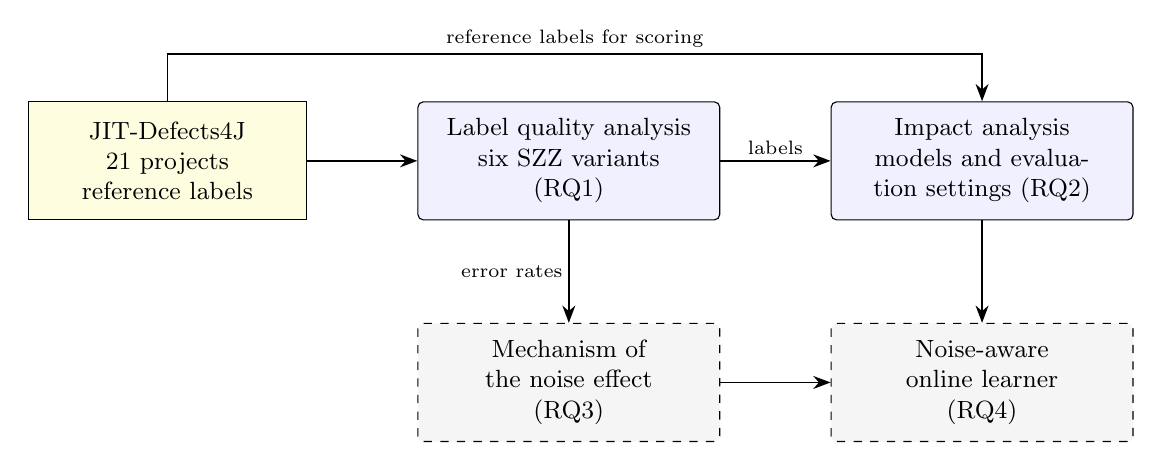
\begin{tikzpicture}[node distance=7mm and 14mm, font=\small,
  box/.style={draw, rounded corners=2pt, align=center, text width=36mm,
              minimum height=15mm, fill=blue!6},
  plan/.style={box, dashed, fill=gray!8},
  data/.style={draw, align=center, text width=33mm, minimum height=15mm, fill=yellow!12},
  arr/.style={-{Stealth[length=2.2mm]}, semithick},
  lab/.style={font=\scriptsize, fill=white, inner sep=1pt}]
\begin{scope}[every node/.append style={execute at begin node=\setstretch{1}}]
\node[data] (ref) {JIT-Defects4J\\21 projects\\reference labels};
\node[box, right=of ref] (s1) {Label quality analysis\\six SZZ variants\\(RQ1)};
\node[box, right=of s1] (s2) {Impact analysis\\models and evaluation settings (RQ2)};
\node[plan, below=13mm of s1] (s3) {Mechanism of the noise effect\\(RQ3)};
\node[plan, below=13mm of s2] (s4) {Noise-aware online learner\\(RQ4)};
\end{scope}
\draw[arr] (ref) -- (s1);
\draw[arr] (s1) -- node[lab, above=1pt] {labels} (s2);
\draw[arr] (s1) -- node[lab, left=1pt] {error rates} (s3);
\draw[arr] (s2) -- (s4);
\draw[arr] (s3) -- (s4);
\draw[arr] (ref.north) -- ++(0,6mm) -| node[lab, pos=0.25, above=1pt]
      {reference labels for scoring} (s2.north);
\end{tikzpicture}
\caption{Overview of the thesis work. The boxes with solid borders belong to
the first stage, which is reported here. The boxes with dashed borders are
planned for the next stage.}
\label{fig:approach}
\end{figure}

\section{Generation of SZZ Labels}\label{sec:szz-generation}

The six SZZ variants of Table~\ref{tab:variants} were executed with PySZZ
(version 2), the implementation released by Rosa et
al.~\cite{rosa2023szzvariants}. An existing implementation was preferred over
writing a new one, because it has been used in earlier studies and its
behaviour is documented. The configuration files supplied with the tool were
used for each variant, with the following settings.

\begin{itemize}[leftmargin=*]
\item The filter that removes candidate commits made after the bug report
date was switched off for all variants, because the dataset does not contain
the dates of the bug reports.
\item For all variants except B-SZZ, commits that modify more than 20 files
are ignored during the blame step. This is the default of the tool and is
intended to skip very large commits such as mass reformatting.
\item MA-SZZ, R-SZZ and L-SZZ use the options of \texttt{git blame} that
detect lines moved within a file and lines moved or copied from other files
changed in the same commit.
\item RA-SZZ analyses only Java source files.
\end{itemize}

The input of the tool is a list of bug-fixing commits. The 5,453 commits of
the dataset whose FIX metric is set were used for this purpose. The same list
was given to all six variants, so that the differences between the label sets
come only from the variants and not from the selection of the bug-fixing
commits.

For every bug-fixing commit the tool returns the list of commits that the
variant considers defect-introducing. These mappings were stored. A commit
was then labelled as defect-introducing by a variant if it appears in the
list of at least one bug-fixing commit, and as clean otherwise. The labels
were joined with the dataset on the commit identifier. All 27,319 commits of
the dataset received a label from each variant. Using the same set of commits
for every variant is important, because precision and recall are not
comparable between variants when they are computed on different subsets.

\section{Analysis of Label Quality}\label{sec:quality-method}

\subsection{Comparison with the reference labels}

For each variant, the SZZ label of every commit is compared with its
reference label. The four possible outcomes are shown in
Table~\ref{tab:confusion}. A commit that is flagged by the variant and is
defect-introducing according to the reference is a true positive (TP). A
commit that is flagged by the variant but is clean according to the reference
is a false positive (FP). A commit that is not flagged but is
defect-introducing according to the reference is a false negative (FN), and a
commit that is clean according to both is a true negative (TN).

\begin{table}[htbp]
\centering\small
\caption{Outcomes of comparing an SZZ label with the reference label.}
\label{tab:confusion}
\begin{tabular}{@{}lcc@{}}
\toprule
 & \multicolumn{2}{c}{Reference label} \\
\cmidrule(l){2-3}
SZZ label & Defect-introducing & Clean \\
\midrule
Defect-introducing & TP & FP \\
Clean & FN & TN \\
\bottomrule
\end{tabular}
\end{table}

From these counts the following measures are computed:
\begin{align}
\text{Precision} &= \frac{TP}{TP+FP}, &
\text{Recall} &= \frac{TP}{TP+FN}, &
F_1 &= \frac{2\cdot\text{Precision}\cdot\text{Recall}}{\text{Precision}+\text{Recall}}.
\end{align}
Precision is the fraction of the commits flagged by the variant that are
defect-introducing according to the reference. Recall is the fraction of the
reference defect-introducing commits that the variant finds. In addition, MCC
and Cohen's $\kappa$ between the SZZ labels and the reference labels are
reported. Both are defined in Section~\ref{sec:measures}.

\subsection{Noise rates}

For the study of label noise it is useful to describe a variant by the
probability with which it changes a reference label. Two rates are defined:
\begin{equation}
\rhoz = \frac{FP}{FP+TN}, \qquad \rhoo = \frac{FN}{FN+TP}.
\label{eq:rho}
\end{equation}
The rate $\rhoz$ is the fraction of the clean commits that the variant labels
as defect-introducing. It is called the false-alarm rate in this report. The
rate $\rhoo$ is the fraction of the defect-introducing commits that the
variant labels as clean. It is called the miss rate and equals one minus the
recall. A noise process that is described by these two rates is known as
class-conditional noise~\cite{natarajan2013noisy}. If both rates were equal,
the noise would be symmetric. Describing each variant by the pair
$(\rhoz,\rhoo)$ shows whether its noise is symmetric and, if not, which type
of error dominates.

Since the two classes have very different sizes, a rate and the corresponding
number of wrong labels must be distinguished. The clean class is about eleven
times larger than the defect-introducing class, so a small value of $\rhoz$
can correspond to a larger number of wrong labels than a large value of
$\rhoo$. Both the rates and the counts are therefore reported.

\subsection{Agreement between variants}

The agreement between two label sets is measured with Cohen's
$\kappa$~\cite{cohen1960kappa},
\begin{equation}
\kappa = \frac{p_o - p_e}{1 - p_e},
\end{equation}
where $p_o$ is the observed fraction of commits on which the two label sets
agree and $p_e$ is the fraction of agreement expected by chance, computed
from the proportions of positive labels in the two sets. The value is
computed for every pair of variants and for every variant with the reference
labels. If the variants made their errors independently of each other, their
mutual agreement would not be much higher than their agreement with the
reference. A much higher mutual agreement indicates that the variants make
the same errors.

\subsection{Variation across projects and sources of false negatives}

All measures are computed for the whole dataset and also for each project
separately, to see how much the quality of the labels varies between
projects.

To understand why the variants miss defect-introducing commits, the false
negatives of each refined variant are divided into two groups by comparing
them with B-SZZ. B-SZZ applies no filtering, so it traces every line changed
by the bug-fixing commits. A false negative of a refined variant that is also
a false negative of B-SZZ was missed already before any filtering. A false
negative of a refined variant that B-SZZ labels correctly was found by the
basic procedure and was then removed by the additional rules of the variant.
The sizes of the two groups show how much of the miss rate of a variant is
caused by its own filtering.

\section{Prediction Models}\label{sec:models}

Three prediction models are used in the impact analysis. They were chosen to
cover different levels of model complexity and both batch and online
learning. All three use the same fourteen change metrics, so that differences
between them are not caused by different inputs.

\subsection{LApredict}

LApredict~\cite{zeng2021lapredict} is a logistic regression model that uses a
single feature, the number of added lines (LA). In this work the feature is
transformed as $\log(1+\mathrm{LA})$ and standardised, and the logistic
regression is trained with class weights that are inversely proportional to
the class frequencies, so that both classes contribute equally to the loss. A
commit is predicted as defect-introducing when the predicted probability is
at least 0.5. The model represents a very simple learner with only two
parameters.

\subsection{Random forest model based on JITLine}

The second model follows the design of
JITLine~\cite{pornprasit2021jitline}: a random forest classifier combined
with oversampling of the minority class. A random
forest~\cite{breiman2001rf} with 100 trees is trained on the fourteen change
metrics, which are transformed as $\mathrm{sign}(x)\log(1+|x|)$ to reduce
their skewness. Before training, the minority class of the training data is
oversampled with SMOTE~\cite{chawla2002smote} until both classes have the
same size. SMOTE creates new minority examples by interpolating between an
existing minority example and one of its nearest minority neighbours (five
neighbours are used).

A random forest produces a probability for each commit, and a decision
threshold is needed to turn it into a class. The threshold is chosen on the
training data so that it maximises the G-mean (Section~\ref{sec:measures}).
To obtain probabilities that are not biased by the model having seen the same
commits, the training data are divided into four consecutive blocks in time
order. A model trained on the first block predicts the second block, a model
trained on the first two blocks predicts the third, and so on. The threshold
is selected on these predictions, and the final model is then trained on the
complete training data.

The original JITLine additionally uses features derived from the tokens of
the changed code. These are not used here, so that all three models work with
the same features. For brevity this model is referred to as JITLine in the
rest of the report. It represents a learner with high capacity, which can fit
complex patterns in the training data.

\subsection{ORB}

The third model is ORB~\cite{cabral2019orb}, an online learner that was
designed for JIT-SDP with verification latency. It is an ensemble that is
updated with one training example at a time. The implementation used in this
work has 20 base learners. Each base learner is a logistic regression model
that is trained by stochastic gradient descent. The features are transformed
in the same way as for the random forest and are standardised with running
estimates of their mean and variance.

When a training example $(x, y)$ arrives, each base learner is updated $k$
times with it, where $k$ is drawn from a Poisson distribution with parameter
$\lambda$. The value of $\lambda$ is what distinguishes the methods of this
family. In Online Bagging $\lambda = 1$. In OOB~\cite{wang2015oob}, $\lambda$
depends on the class of the example and on the current proportion $r_1$ of
positive examples, which is tracked as a decayed average,
\begin{equation}
r_1 \leftarrow \delta\, r_1 + (1-\delta)\,I(y=1), \qquad \delta = 0.99,
\end{equation}
where $I(y=1)$ is 1 if the example is positive and 0 otherwise. The rate is
then
\begin{equation}
\lambda_{\mathrm{OOB}} =
\begin{cases}
(1-r_1)/r_1 & \text{if } y=1 \text{ and } r_1 < 0.5,\\
r_1/(1-r_1) & \text{if } y=0 \text{ and } r_1 > 0.5,\\
1 & \text{otherwise.}
\end{cases}
\label{eq:oob}
\end{equation}
For example, if 10\% of the recent training examples are positive, a positive
example is presented on average nine times to each base learner.

ORB multiplies this rate by a boosting factor $b$ that depends on the recent
predictions of the model. Let $\bar{p}$ be a moving average of the
predictions (1 for defect-introducing, 0 for clean), which is updated after
every prediction as $\bar{p} \leftarrow \theta\,\bar{p} + (1-\theta)\,\hat{y}$
with $\theta = 0.4$. If the model predicts the positive class less often than
the proportion of positive examples it has seen ($\bar{p} < r_1$), positive
training examples are boosted. If it predicts the positive class more often
($\bar{p} > r_1$), negative training examples are boosted:
\begin{equation}
b =
\begin{cases}
l_0\,\dfrac{m^{\bar{p}} - m^{r_1}}{1 - m^{r_1}} + 1 & \text{if } y=1 \text{ and } \bar{p} < r_1,\\[2.2ex]
l_1\,\dfrac{n^{1-\bar{p}} - n^{1-r_1}}{1 - n^{1-r_1}} + 1 & \text{if } y=0 \text{ and } \bar{p} > r_1,\\[1.6ex]
1 & \text{otherwise,}
\end{cases}
\label{eq:orb}
\end{equation}
with the parameter values $l_0 = 10$, $l_1 = 12$, $m = 1.5$ and $n = 3$
proposed by the authors of ORB~\cite{cabral2019orb}. The final rate is
$\lambda = \lambda_{\mathrm{OOB}} \cdot b$. A commit is predicted as
defect-introducing when the majority of the base learners predict it so.

It can be seen from Equations~\ref{eq:oob} and~\ref{eq:orb} that the amount
of oversampling depends on the number of positive labels received and on the
predictions of the model, but not on whether the labels are correct. ORB
represents the online learners that are used when the commit stream is
processed in a realistic way.

\section{Evaluation Settings}\label{sec:settings}

The models are evaluated in four settings, which are illustrated in
Figure~\ref{fig:settings}. They are ordered from the least to the most
realistic.

\begin{figure}[htbp]
\centering
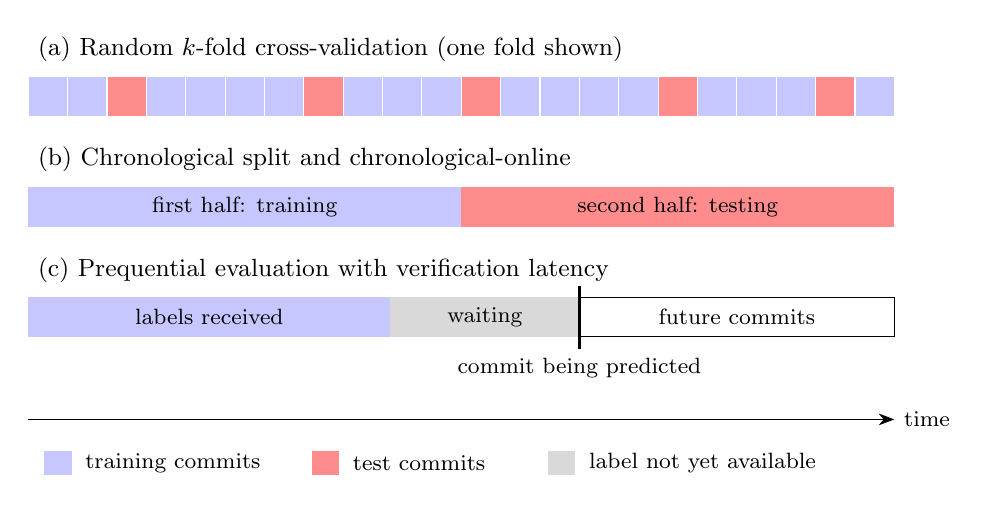
\begin{tikzpicture}[font=\footnotesize, x=1cm, y=1cm]
\def\w{11}
% (a) random k-fold
\node[anchor=west, font=\small] at (0,5.55) {(a) Random $k$-fold cross-validation (one fold shown)};
\foreach \i in {0,...,21} {
  \pgfmathtruncatemacro{\istest}{(\i==2 || \i==7 || \i==11 || \i==16 || \i==20) ? 1 : 0}
  \ifnum\istest=1
    \fill[red!45] (\i*0.5,4.7) rectangle ++(0.5,0.5);
  \else
    \fill[blue!22] (\i*0.5,4.7) rectangle ++(0.5,0.5);
  \fi
  \draw[white] (\i*0.5,4.7) rectangle ++(0.5,0.5);
}
% (b) chronological
\node[anchor=west, font=\small] at (0,4.15) {(b) Chronological split and chronological-online};
\fill[blue!22] (0,3.3) rectangle (5.5,3.8);
\fill[red!45] (5.5,3.3) rectangle (\w,3.8);
\node at (2.75,3.55) {first half: training};
\node at (8.25,3.55) {second half: testing};
% (c) prequential
\node[anchor=west, font=\small] at (0,2.75) {(c) Prequential evaluation with verification latency};
\fill[blue!22] (0,1.9) rectangle (4.6,2.4);
\fill[gray!30] (4.6,1.9) rectangle (7.0,2.4);
\draw (7.0,1.9) rectangle (\w,2.4);
\draw[thick] (7.0,1.75) -- (7.0,2.55);
\node at (2.3,2.15) {labels received};
\node at (5.8,2.15) {waiting};
\node at (9.0,2.15) {future commits};
\node[anchor=north] at (7.0,1.75) {commit being predicted};
% time axis and legend
\draw[-{Stealth[length=2mm]}] (0,0.85) -- (\w,0.85) node[right] {time};
\fill[blue!22] (0.2,0.15) rectangle ++(0.35,0.3); \node[anchor=west] at (0.6,0.3) {training commits};
\fill[red!45] (3.6,0.15) rectangle ++(0.35,0.3); \node[anchor=west] at (4.0,0.3) {test commits};
\fill[gray!30] (6.6,0.15) rectangle ++(0.35,0.3); \node[anchor=west] at (7.0,0.3) {label not yet available};
\end{tikzpicture}
\caption{The evaluation settings. The commits of a project are ordered by
time from left to right.}
\label{fig:settings}
\end{figure}

\paragraph{Random $k$-fold cross-validation.} The commits of a project are
divided at random into ten folds, stratified by the training label. Each fold
is used once for testing while the model is trained on the other nine. The
order of the commits is ignored, so the model is trained on commits that are
both older and newer than the test commits. This setting is included because
it is widely used in the literature. It is applied to the two batch models.

\paragraph{Chronological split.} The commits of a project are ordered by
time. The model is trained on the first half and tested on the second half.
The model never sees commits from the future, but it is assumed that the
labels of all training commits are known at the time of training. This
setting is also applied to the two batch models.

\paragraph{Chronological-online.} This setting uses the same split for ORB.
The online learner processes the commits of the first half one by one with
their labels and is then kept fixed while it predicts the second half. It
makes it possible to compare ORB with the batch models on the same test
commits, and to see how ORB behaves when it is not updated during testing.

\paragraph{Prequential evaluation with verification latency.} The commits are
processed in time order. Each commit is first predicted by the current model.
Its label is given to the model for training only at the time at which it
would have become available in practice. The details are given in the next
section. The model is updated continuously over the whole stream. This
setting is the closest to the actual use of a JIT-SDP model and is applied to
ORB.

\section{Simulation of Verification Latency}\label{sec:latency-method}

In the prequential setting the labels are delivered to the learner according
to the procedure of Cabral et al.~\cite{cabral2019orb} with a waiting period
of $W = 90$ days. Let $t$ be the time of a commit. Four cases are
distinguished according to the training label of the commit and the time of
the bug-fixing commit linked to it (Section~\ref{sec:latency-data}). They are
shown in Figure~\ref{fig:latency-cases}.

\begin{enumerate}[leftmargin=*]
\item The commit is clean according to the training labels. Nothing is known
about it until the waiting period has passed. At time $t+W$ it is given to
the learner as a clean example.
\item The commit is defect-introducing and its fix is made before $t+W$. It
is given to the learner as a defect-introducing example at the time of the
fix.
\item The commit is defect-introducing and its fix is made after $t+W$. At
time $t+W$ no defect is known yet, so the commit is given to the learner as
a clean example. At the time of the fix it is given again, this time as a
defect-introducing example.
\item The commit is defect-introducing according to the training labels, but
no fix date is available for it. It is given to the learner as a clean
example at $t+W$ and is never corrected.
\end{enumerate}

\begin{figure}[htbp]
\centering
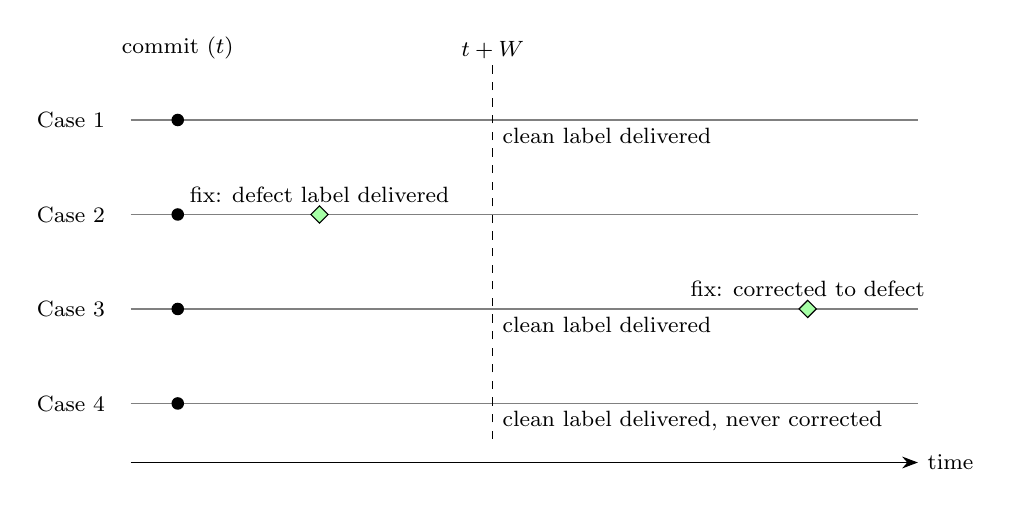
\begin{tikzpicture}[font=\footnotesize, x=1cm, y=1cm,
  ev/.style={circle, fill=black, inner sep=1.6pt},
  fix/.style={diamond, draw, fill=green!35, inner sep=1.6pt}]
\foreach \y/\lab in {3.6/Case 1, 2.4/Case 2, 1.2/Case 3, 0/Case 4} {
  \draw[gray] (1.6,\y) -- (11.6,\y);
  \node[anchor=east] at (1.4,\y) {\lab};
  \node[ev] at (2.2,\y) {};
}
\draw[dashed] (6.2,-0.45) -- (6.2,4.3);
\node[anchor=south] at (2.2,4.25) {commit ($t$)};
\node[anchor=south] at (6.2,4.25) {$t+W$};
% case 1
\node[anchor=north west, inner sep=2pt] at (6.25,3.58) {clean label delivered};
% case 2
\node[fix] at (4.0,2.4) {};
\node[anchor=south, inner sep=3pt] at (4.0,2.44) {fix: defect label delivered};
% case 3
\node[anchor=north west, inner sep=2pt] at (6.25,1.18) {clean label delivered};
\node[fix] at (10.2,1.2) {};
\node[anchor=south, inner sep=3pt] at (10.2,1.24) {fix: corrected to defect};
% case 4
\node[anchor=north west, inner sep=2pt] at (6.25,-0.02) {clean label delivered, never corrected};
\draw[-{Stealth[length=2mm]}] (1.6,-0.75) -- (11.6,-0.75) node[right] {time};
\end{tikzpicture}
\caption{Delivery of training labels under verification latency. In case 3
the learner first receives a wrong clean label, which is corrected when the
defect is fixed.}
\label{fig:latency-cases}
\end{figure}

Cases 3 and 4 are the ones in which the learner is trained on a wrong label
because of the delay. In case 3 the error is temporary. In case 4 it is
permanent. These errors occur with every label source, including the
reference labels, and they concern only defect-introducing commits. They add
to whatever errors the labels themselves contain.

The prediction for a commit is made at time $t$ and is scored at once, using
the label against which the model is evaluated (Section~\ref{sec:scoring}).
The scoring is not delayed, because its purpose is to measure the quality of
the predictions and not to simulate what a user of the model would know.
Algorithm~\ref{alg:prequential} summarises the procedure.

\begin{algorithm}[htbp]
\caption{Prequential evaluation with verification latency}
\label{alg:prequential}
\begin{algorithmic}[1]
\Require commits $c_1,\dots,c_N$ of a project in time order, with features
$x_i$, time $t_i$, training label $y_i$, evaluation label $e_i$ and fix time
$f_i$ (if available); waiting period $W$; online learner $M$
\State $Q \gets$ empty priority queue of pending training examples, ordered by delivery time
\For{$i = 1$ to $N$}
  \While{$Q$ is not empty and the earliest delivery time in $Q$ is at most $t_i$}
    \State remove the earliest example $(x_j, y)$ from $Q$ and update $M$ with it
  \EndWhile
  \State $\hat{y}_i \gets$ prediction of $M$ for $x_i$
  \State update the evaluation measures with $(e_i, \hat{y}_i)$
  \If{$y_i = 1$ and $f_i$ is available}
    \If{$f_i \le t_i + W$}
      \State add $(x_i, 1)$ to $Q$ with delivery time $f_i$
    \Else
      \State add $(x_i, 0)$ to $Q$ with delivery time $t_i + W$
      \State add $(x_i, 1)$ to $Q$ with delivery time $f_i$
    \EndIf
  \Else
    \State add $(x_i, 0)$ to $Q$ with delivery time $t_i + W$
  \EndIf
\EndFor
\end{algorithmic}
\end{algorithm}

\section{Scoring of the Predictions}\label{sec:scoring}

The predictions of a model can be compared with two different labels.

\paragraph{Scoring against the reference labels.} The predictions are
compared with the reference labels of the test commits. These labels are
never used for training when the model is trained on SZZ labels. The result
shows how well the model identifies the commits that are defect-introducing
according to the best available standard. This is the main way of scoring in
this work, and it is used unless stated otherwise.

\paragraph{Scoring against the training labels.} The predictions are
compared with the labels of the same SZZ variant that was used for training.
This is what is done in the literature, where only one set of labels is
available. It is called \emph{self-scoring} in this report.

For a model trained on SZZ labels both scores are computed from the same
predictions. The difference between them shows how much the usual way of
scoring overestimates or underestimates the performance with respect to the
reference. For a model trained on the reference labels the two scores are the
same by definition.

\section{Performance Measures}\label{sec:measures}

\subsection{MCC and G-mean}

The main performance measure is the Matthews correlation
coefficient~\cite{matthews1975mcc},
\begin{equation}
\mathrm{MCC} = \frac{TP\cdot TN - FP\cdot FN}
{\sqrt{(TP+FP)(TP+FN)(TN+FP)(TN+FN)}},
\end{equation}
where the four counts are now obtained by comparing the predictions with the
evaluation labels. MCC ranges from $-1$ to $+1$. It is 0 for a model that
predicts at random or assigns all commits to one class, and it is high only
if the model performs well on both classes. It was chosen because of the
class imbalance: a model that predicts every commit as clean would reach an
accuracy of 91.5\% on this dataset but has an MCC of 0. MCC has also been
recommended for defect prediction in place of the
F-measure~\cite{yao2020mcc,chicco2020mcc}.

As a second measure the G-mean is reported, which is the geometric mean of
the recall on the two classes,
\begin{equation}
\text{G-mean} = \sqrt{\frac{TP}{TP+FN}\cdot\frac{TN}{TN+FP}}.
\end{equation}
It is commonly used in online JIT-SDP~\cite{cabral2019orb} and becomes zero
when one of the classes is not recognised at all.

\subsection{Measures in the prequential setting}

In the prequential setting the performance is not a single value, since the
model changes during the stream. The usual practice is to compute the
measures from a confusion matrix with a fading
factor~\cite{gama2013prequential}. Before each update, the four counts are
multiplied by a factor $f < 1$, and then the count that corresponds to the
new prediction is increased by one. Older predictions thus have less weight.
With $f = 0.99$, which is used here, the weights add up to $1/(1-f) = 100$,
so the matrix effectively describes the last hundred commits.

Let $\mathrm{MCC}_i$ be the MCC computed from the faded matrix after the
$i$-th commit of a stream of $N$ commits. Two summaries of this sequence are
used.

\begin{itemize}[leftmargin=*]
\item The \emph{terminal} value $\mathrm{MCC}_N$ is the value at the end of
the stream. It reflects the performance on roughly the last hundred commits.
\item The \emph{time-averaged} value $\frac{1}{N}\sum_{i=1}^{N}\mathrm{MCC}_i$
is the mean over the whole stream.
\end{itemize}

The terminal value depends on a small part of the stream, which contains on
average only about eight defect-introducing commits. It therefore varies
strongly from project to project. The standard deviation of the project-level
values is 0.092 for the terminal value and 0.051 for the time-averaged value.
Because it is more stable, the time-averaged value is used as the primary
summary in this work, and the terminal value is reported as a secondary one.
The convergence result of Gama et al.\ for the faded error rate does not
carry over to MCC, which is not a sum of per-example losses, so neither
summary can claim to be the standard one. All results of the prequential
setting are therefore given for both summaries, and the sensitivity of the
conclusions to the fading factor is examined separately
(Section~\ref{sec:robustness}).

\section{Statistical Analysis}\label{sec:stats}

\subsection{Unit of analysis}

Each configuration is run with ten random seeds on each of the 21 projects.
The seeds affect the random forest, the oversampling, the assignment of
commits to folds and the Poisson draws of ORB. Runs with different seeds on
the same project are not independent observations, because they use the same
data. For every configuration the results of the ten seeds are therefore
averaged for each project first, and the statistical tests are carried out on
the 21 project-level values. All comparisons are paired by project: the two
conditions that are compared are always evaluated on the same projects.

\subsection{Test and effect sizes}

Let $d_1,\dots,d_{21}$ be the differences between two conditions for the 21
projects. The following quantities are reported for each comparison.

\paragraph{Wilcoxon signed-rank test.} The null hypothesis that the
differences are symmetric around zero is tested with the Wilcoxon signed-rank
test~\cite{wilcoxon1945}. The absolute differences are ranked, and the sum
$W^{+}$ of the ranks of the positive differences and the sum $W^{-}$ of the
ranks of the negative differences are computed. The test is non-parametric
and does not assume that the differences are normally distributed, which
cannot be assumed for MCC values of 21 projects.

\paragraph{Rank-biserial correlation.} As a measure of how consistently the
projects point in the same direction, the matched-pairs rank-biserial
correlation is used,
\begin{equation}
r = \frac{W^{+} - W^{-}}{W^{+} + W^{-}}.
\end{equation}
It is $+1$ if all differences are positive, $-1$ if all are negative, and 0
if the positive and negative ranks balance. Values of 0.1, 0.3 and 0.5 are
commonly regarded as small, medium and large.

\paragraph{Hodges--Lehmann estimate.} The size of the difference is
estimated with the Hodges--Lehmann estimator~\cite{hodges1963}, which is the
median of all pairwise averages $(d_i + d_j)/2$ with $i \le j$. It is the
estimate of location that belongs to the signed-rank test and is less
sensitive to single extreme projects than the mean.

\paragraph{Confidence interval.} A 95\% confidence interval for the
Hodges--Lehmann estimate is obtained with the percentile
bootstrap~\cite{efron1979bootstrap}. The 21 projects are resampled with
replacement 10,000 times, the estimate is recomputed for each resample, and
the 2.5th and 97.5th percentiles of the resulting values are taken as the
limits.

\subsection{Correction for multiple comparisons}

In total 74 tests are carried out in the impact analysis. They belong to the
five families listed in Table~\ref{tab:families}. When many tests are made,
some of them are expected to be significant by chance. The $p$-values are
therefore adjusted with the method of Holm~\cite{holm1979}. For $m$ tests
with ordered $p$-values $p_{(1)} \le \dots \le p_{(m)}$, the adjusted value
of the $i$-th one is
\begin{equation}
\tilde{p}_{(i)} = \max_{j \le i}\,\min\bigl(1,\,(m-j+1)\,p_{(j)}\bigr).
\end{equation}

The correction is applied in two ways. First, it is applied within each
family of related tests. Second, it is applied to all 74 tests together. The
second correction is stricter. It is reported because the families were
defined during the analysis and not before it, so that it could be argued
that the grouping was chosen favourably. A result that remains significant
after the correction over all tests does not depend on how the families were
formed. The main conclusions of this report are based on this global
correction. A significance level of 0.05 is used.

\begin{table}[htbp]
\centering\small
\caption{Families of statistical tests in the impact analysis.}
\label{tab:families}
\begin{tabularx}{\linewidth}{@{}>{\raggedright\arraybackslash}p{38mm}>{\raggedright\arraybackslash}Xr@{}}
\toprule
Family & Comparison & Tests \\
\midrule
Evaluation setting & Random $k$-fold against chronological split, for each
batch model and label source & 14 \\
Scoring & Self-scored against reference-scored, for each model, SZZ variant
and evaluation setting (for the prequential setting with both summaries) & 42 \\
Label source & ORB trained on reference labels against ORB trained on each
SZZ variant, prequential setting (both summaries) & 12 \\
Learner & Each batch model against ORB on the chronological split & 4 \\
Online setting & ORB in the chronological-online setting against ORB in the
prequential setting & 2 \\
\midrule
Total & & 74 \\
\bottomrule
\end{tabularx}
\end{table}

\section{Additional Analyses}\label{sec:additional-method}

Besides the main experiment, some additional analyses were carried out to
examine specific questions that arose from the results. Their design is
described here, and their results are given in Chapter~\ref{ch:results}.

\paragraph{Predictability of SZZ errors.} To examine whether the false
positives of SZZ have properties that a model can learn, a classifier is
trained to separate the false positives of B-SZZ from its true positives.
Only the 8,060 commits flagged by B-SZZ are used. For each project they are
split chronologically into two halves, and a random forest with 100 trees is
trained on the first half with the fourteen change metrics. Its area under
the ROC curve (AUC) on the second half is compared with the AUC of the same
procedure when the training labels are randomly permuted. Five seeds are
used.

\paragraph{Separation of label delay and model adaptation.} The
chronological-online and prequential settings differ in two respects: whether
the labels are delayed, and whether the model continues to learn during
testing. To separate the two, ORB is evaluated in all four combinations of
these factors with reference labels: frozen or adaptive learner, and
immediate or delayed labels. In all four cases the performance is computed on
the second half of the stream with the ordinary (not faded) MCC, so that the
cells are directly comparable.

\paragraph{Sensitivity to the prequential summary.} The comparison of label
sources in the prequential setting is repeated for five values of the fading
factor (0.90, 0.95, 0.99, 0.995 and 0.999) and for four lengths of an initial
warm-up period that is excluded from the average (0\%, 5\%, 10\% and 25\% of
the stream).

\paragraph{Availability of arrival times.} For the reference labels, an
arrival time is available for only 67.8\% of the defect-introducing commits
(Section~\ref{sec:latency-data}), whereas it is available for all commits
flagged by the SZZ variants. To check whether this difference influences the
comparison, the missing arrival times of the reference labels are imputed by
drawing latencies at random from the observed latency distribution, and the
evaluation is repeated.

\paragraph{Exclusion of small projects.} Some projects contain few
defect-introducing commits. The main comparisons are repeated after
excluding the projects with fewer than 25 defect-introducing commits in the
second half of their history, which leaves 13 projects.

\section{Experimental Setup}

The experiment of the impact analysis combines the three models with the
seven label sources, the evaluation settings applicable to each model and
the two ways of scoring. Table~\ref{tab:design} summarises the factors. For
each project and seed there are 78 configurations: each of the two batch
models is evaluated in two settings with seven label sources scored against
the reference and six scored against the training labels, and the same holds
for ORB with its two settings. With 21 projects and ten seeds this gives
$78 \times 21 \times 10 = 16{,}380$ evaluation runs.

\begin{table}[htbp]
\centering\small
\caption{Factors of the experiment in the impact analysis.}
\label{tab:design}
\begin{tabularx}{\linewidth}{@{}l>{\raggedright\arraybackslash}X@{}}
\toprule
Factor & Levels \\
\midrule
Model & LApredict, JITLine (batch models); ORB (online model) \\
Training labels & Reference labels; labels of B-SZZ, AG-SZZ, MA-SZZ, L-SZZ,
R-SZZ and RA-SZZ \\
Evaluation setting & Random 10-fold cross-validation and chronological split
(batch models); chronological-online and prequential with verification
latency (ORB) \\
Scoring & Against the reference labels; against the training labels \\
Projects & 21 \\
Random seeds & 10 \\
\bottomrule
\end{tabularx}
\end{table}

The experiments were implemented in Python 3.13 with scikit-learn 1.9.0 for
the batch models, imbalanced-learn 0.14.2 for SMOTE, and NumPy, pandas and
SciPy for the data handling and the statistical tests. The online learner
and the prequential evaluation were implemented for this work. The versions
of all libraries are fixed in the project, so that the results can be
regenerated exactly.

Two measures were taken to keep the results consistent. First, every table
and figure in this report is produced by a script from the stored outputs of
the experiments. Second, before the experiments of the impact analysis are
run, a check recomputes the counts of Table~\ref{tab:confusion} from the
label columns of the experimental data and compares them with the results of
the label quality analysis. This ensures that the models are trained on
exactly the labels whose quality is reported.

\section{Summary}

In the first study, six SZZ variants are run with PySZZ on 5,453 bug-fixing
commits, and their labels are compared with the reference labels in terms of
precision, recall, noise rates and agreement. In the second study, three
models of different complexity are trained on seven label sources and
evaluated in four settings, from random cross-validation to prequential
evaluation with verification latency. The predictions are scored against the
reference labels and against the training labels. The comparisons are tested
at the level of projects with the Wilcoxon signed-rank test, and the
$p$-values are corrected for multiple comparisons.

% ============================================================================
\chapter{Results and Discussion}\label{ch:results}
% ============================================================================

This chapter presents the results of the first stage of the thesis.
Section~\ref{sec:res-quality} gives the results of the label quality analysis
and answers RQ1. Section~\ref{sec:res-impact} gives the results of the impact
analysis and answers RQ2. Section~\ref{sec:res-summary} summarises the
findings.

\section{Quality of the SZZ Labels}\label{sec:res-quality}

\subsection{Overall quality}

Table~\ref{tab:counts} shows, for each variant, the number of commits it
flags as defect-introducing and the outcome of the comparison with the
reference labels. Table~\ref{tab:quality} gives the measures computed from
these counts. All numbers refer to the same 27,319 commits, of which 2,332
are defect-introducing and 24,987 are clean according to the reference.

\begin{table}[htbp]
\centering\small
\caption{Number of commits flagged by each SZZ variant and comparison with
the reference labels.}
\label{tab:counts}
\begin{tabular}{@{}lrrrrrr@{}}
\toprule
Variant & Flagged & \% of commits & TP & FP & FN & TN \\
\midrule
B-SZZ & 8,060 & 29.5 & 1,495 & 6,565 & 837 & 18,422 \\
AG-SZZ & 5,876 & 21.5 & 1,090 & 4,786 & 1,242 & 20,201 \\
MA-SZZ & 6,154 & 22.5 & 1,124 & 5,030 & 1,208 & 19,957 \\
L-SZZ & 2,287 & 8.4 & 622 & 1,665 & 1,710 & 23,322 \\
R-SZZ & 3,015 & 11.0 & 699 & 2,316 & 1,633 & 22,671 \\
RA-SZZ & 5,553 & 20.3 & 1,022 & 4,531 & 1,310 & 20,456 \\
\bottomrule
\end{tabular}
\end{table}

\begin{table}[htbp]
\centering\small
\caption{Quality of the SZZ labels with respect to the reference labels. The
best value in each column is shown in bold.}
\label{tab:quality}
\begin{tabular}{@{}lccccccc@{}}
\toprule
Variant & Precision & Recall & $F_1$ & MCC & $\kappa$ & $\rhoz$ & $\rhoo$ \\
\midrule
B-SZZ & 0.186 & \textbf{0.641} & \textbf{0.288} & \textbf{0.232} & 0.179 & 0.263 & \textbf{0.359} \\
AG-SZZ & 0.186 & 0.467 & 0.266 & 0.188 & 0.163 & 0.192 & 0.533 \\
MA-SZZ & 0.183 & 0.482 & 0.265 & 0.188 & 0.161 & 0.201 & 0.518 \\
L-SZZ & \textbf{0.272} & 0.267 & 0.269 & 0.202 & \textbf{0.202} & \textbf{0.067} & 0.733 \\
R-SZZ & 0.232 & 0.300 & 0.262 & 0.185 & 0.183 & 0.093 & 0.700 \\
RA-SZZ & 0.184 & 0.438 & 0.259 & 0.178 & 0.158 & 0.181 & 0.562 \\
\bottomrule
\end{tabular}
\end{table}

The following observations can be made from these tables and from
Figure~\ref{fig:szz-quality}.

\paragraph{The precision of all variants is low.} The precision lies between
0.183 and 0.272. This means that between 72.8\% and 81.7\% of the commits
that a variant labels as defect-introducing are clean according to the
reference. B-SZZ flags 8,060 commits, which is 29.5\% of all commits, whereas
only 8.54\% of the commits are defect-introducing according to the reference.
The refined variants flag fewer commits, but their precision is not higher
than that of B-SZZ, with the exception of L-SZZ and R-SZZ, which keep only
one candidate per bug-fixing commit.

\paragraph{The recall decreases with every refinement.} B-SZZ finds 64.1\%
of the reference defect-introducing commits. AG-SZZ and MA-SZZ find about
47\% to 48\%, RA-SZZ 43.8\%, R-SZZ 30.0\% and L-SZZ only 26.7\%. The two
variants with the highest precision are thus the ones that miss the most
defects.

\paragraph{The two types of error are not balanced, and the balance differs
between the variants.} Figure~\ref{fig:szz-quality}(b) plots the false-alarm
rate $\rhoz$ against the miss rate $\rhoo$. The variants lie along a line from
the upper left to the lower right. B-SZZ has the highest false-alarm rate
(0.263) and the lowest miss rate (0.359). L-SZZ and R-SZZ have low
false-alarm rates (0.067 and 0.093) and very high miss rates (0.733 and
0.700). AG-SZZ, MA-SZZ and RA-SZZ lie in between. In no case are the two
rates equal, so the noise of SZZ cannot be described as symmetric. The noise
also cannot be described by a single pair of rates for SZZ in general, because
the pair depends strongly on the variant.

\paragraph{No variant is better than the others on all measures.} B-SZZ has
the highest recall, $F_1$ and MCC. L-SZZ has the highest precision and
$\kappa$. The $F_1$ values of the six variants are almost the same (0.259 to
0.288), although the variants behave very differently. A comparison of SZZ
variants on a single summary measure can therefore be misleading.

\begin{figure}[htbp]
\centering
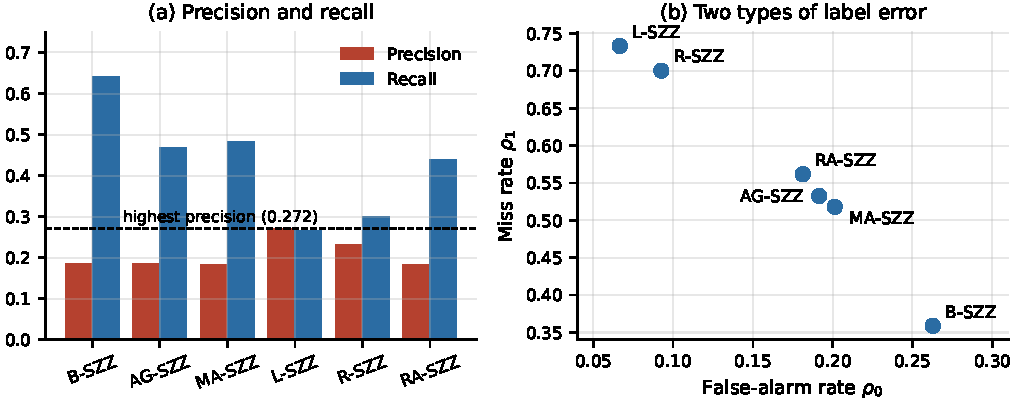
\includegraphics[width=\linewidth]{fig_szz_quality}
\caption{(a) Precision and recall of the SZZ variants with respect to the
reference labels. (b) False-alarm rate and miss rate of the variants.}
\label{fig:szz-quality}
\end{figure}

Figure~\ref{fig:szz-volume} shows the same results as numbers of commits.
Because the clean class is much larger than the defect-introducing class,
the number of false positives exceeds the number of false negatives for five
of the six variants, even for those whose miss rate is much higher than their
false-alarm rate. For B-SZZ there are 6,565 false positives and 837 false
negatives, a ratio of about eight to one. Only for L-SZZ are the two numbers
approximately equal (1,665 and 1,710). When the effect of the two types of
error on a learner is studied, it will therefore be necessary to distinguish
between the effect of a single wrong label of each type and the effect of
their different numbers.

\begin{figure}[htbp]
\centering
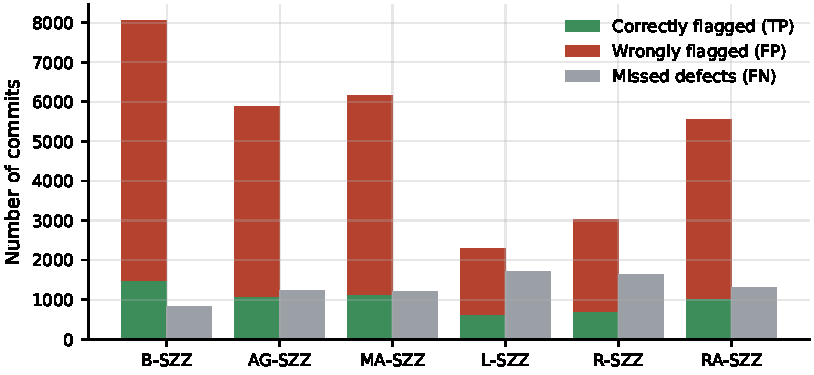
\includegraphics[width=0.8\linewidth]{fig_szz_volume}
\caption{Number of correctly flagged, wrongly flagged and missed commits for
each variant.}
\label{fig:szz-volume}
\end{figure}

\subsection{Variation across projects}

Table~\ref{tab:perproject} gives the minimum, median and maximum of precision
and recall over the 21 projects, and Figure~\ref{fig:szz-perproject} shows
the distributions. The quality of the labels varies widely between projects.
The recall of B-SZZ is 0.220 in opennlp and 0.919 in commons-beanutils. Its
precision is 0.056 in commons-collections and 0.386 in ant-ivy. For AG-SZZ
the recall ranges from 0.074 to 0.819. The values for the whole dataset in
Table~\ref{tab:quality} are thus not representative of an individual
project. This is one of the reasons why the statistical comparisons in the
impact analysis are made per project.

\begin{table}[htbp]
\centering\small
\caption{Minimum, median and maximum of precision and recall over the 21
projects.}
\label{tab:perproject}
\begin{tabular}{@{}lcccccc@{}}
\toprule
 & \multicolumn{3}{c}{Precision} & \multicolumn{3}{c}{Recall} \\
\cmidrule(lr){2-4}\cmidrule(l){5-7}
Variant & Min. & Median & Max. & Min. & Median & Max. \\
\midrule
B-SZZ & 0.056 & 0.199 & 0.386 & 0.220 & 0.700 & 0.919 \\
AG-SZZ & 0.053 & 0.222 & 0.325 & 0.074 & 0.389 & 0.819 \\
MA-SZZ & 0.053 & 0.188 & 0.325 & 0.098 & 0.417 & 0.819 \\
L-SZZ & 0.072 & 0.271 & 0.491 & 0.080 & 0.245 & 0.432 \\
R-SZZ & 0.058 & 0.213 & 0.450 & 0.061 & 0.250 & 0.552 \\
RA-SZZ & 0.042 & 0.213 & 0.328 & 0.110 & 0.361 & 0.789 \\
\bottomrule
\end{tabular}
\end{table}

\begin{figure}[htbp]
\centering
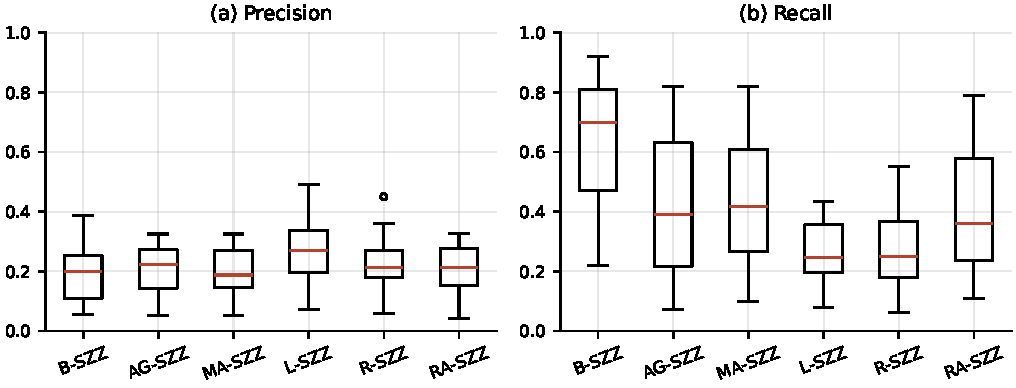
\includegraphics[width=\linewidth]{fig_szz_perproject}
\caption{Distribution of precision and recall of each variant over the 21
projects.}
\label{fig:szz-perproject}
\end{figure}

\subsection{Agreement between the variants}

Figure~\ref{fig:kappa} shows Cohen's $\kappa$ for every pair of label sets.
The first row and column give the agreement of each variant with the
reference labels, and the remaining cells give the agreement between
variants.

\begin{figure}[htbp]
\centering
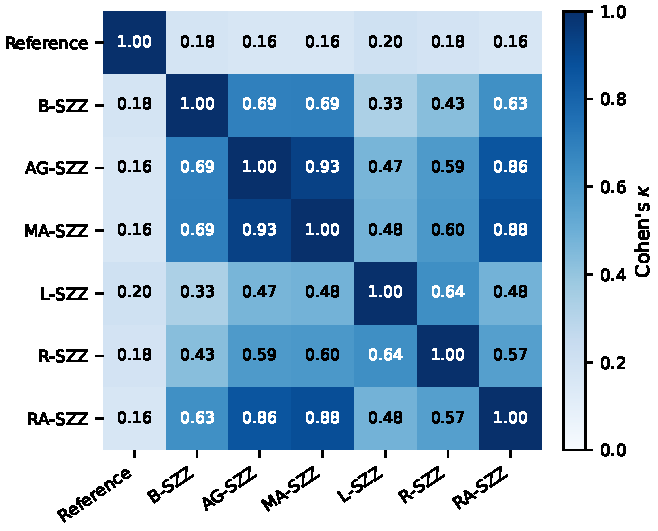
\includegraphics[width=0.68\linewidth]{fig_kappa}
\caption{Cohen's $\kappa$ between the reference labels and the labels of the
six SZZ variants.}
\label{fig:kappa}
\end{figure}

The agreement of the variants with the reference is between 0.158 and 0.202,
which is slight agreement in the terms of Landis and
Koch~\cite{landis1977kappa}. The agreement among the variants is much higher.
AG-SZZ, MA-SZZ and RA-SZZ agree with each other at 0.86 to 0.93, which is
almost perfect agreement. B-SZZ agrees with these three at 0.63 to 0.70.
L-SZZ and R-SZZ agree with each other at 0.64 and with the others at 0.33 to
0.60. Two groups can be recognised: the variants that filter lines (AG-SZZ,
MA-SZZ, RA-SZZ) and the variants that select a single candidate (L-SZZ,
R-SZZ).

Even the lowest agreement between two variants (0.33) is higher than the
highest agreement of any variant with the reference (0.20). The variants are
therefore much more similar to each other than to the reference. This is
plausible, since all of them start from the same bug-fixing commits and use
the same blame mechanism, so they are affected by tangled changes in the
same way.

This has a practical implication. When two SZZ variants or implementations
produce similar labels, this is sometimes taken as an indication that the
labels are reliable. The present result shows that this conclusion is not
justified. The variants agree to a large extent on commits that are wrongly
flagged. In total, 8,821 commits are flagged by at least one variant and
1,534 by all six. Of the 2,332 reference defect-introducing commits, 1,581
(67.8\%) are flagged by at least one variant, only 450 (19.3\%) are flagged
by all six, and 751 (32.2\%) are not flagged by any variant.

\subsection{Sources of the false negatives}\label{sec:fn-sources}

The high miss rates of the refined variants raise the question of where the
missed commits are lost. As explained in Section~\ref{sec:reference}, every
reference defect-introducing commit can be reached by blame, so the losses
cannot be explained by defects that leave no traceable line.
Table~\ref{tab:fn} divides the false negatives of each refined variant into
those that B-SZZ also misses and those that B-SZZ finds.

\begin{table}[htbp]
\centering\small
\caption{False negatives of the refined variants, divided according to
whether B-SZZ also misses the commit. The last column gives the share of the
1,495 true positives of B-SZZ that the variant no longer flags.}
\label{tab:fn}
\begin{tabular}{@{}lrrrr@{}}
\toprule
Variant & False negatives & Also missed & Found by B-SZZ & Share of B-SZZ true \\
 & & by B-SZZ & but removed & positives removed \\
\midrule
AG-SZZ & 1,242 & 765 (62\%) & 477 (38\%) & 31.9\% \\
MA-SZZ & 1,208 & 763 (63\%) & 445 (37\%) & 29.8\% \\
RA-SZZ & 1,310 & 765 (58\%) & 545 (42\%) & 36.5\% \\
R-SZZ & 1,633 & 808 (49\%) & 825 (51\%) & 55.2\% \\
L-SZZ & 1,710 & 807 (47\%) & 903 (53\%) & 60.4\% \\
\bottomrule
\end{tabular}
\end{table}

Two sources of roughly similar size can be seen.

The first source is common to all variants. B-SZZ itself misses 837 reference
defect-introducing commits, and between 763 and 808 of them are also missed
by each refined variant. These commits are not reached although B-SZZ traces
every changed line of the bug-fixing commits. Since both procedures use
blame, the difference must lie in the starting points of the tracing, that
is, in the set of bug-fixing commits and in the lines from which the tracing
starts. In this work the bug-fixing commits were taken from the FIX metric of
the dataset, while the reference labels were derived from the validated
bug-fixing commits of LLTC4J, and the two sets need not be identical. This
part of the miss rate can therefore not be attributed to the SZZ variants
alone.

The second source is the filtering of the variants. Between 445 and 903 of
the commits that B-SZZ labels correctly are removed again by the refined
variants. AG-SZZ, MA-SZZ and RA-SZZ remove about 30\% to 37\% of the true
positives of B-SZZ. R-SZZ and L-SZZ remove more than half of them (55.2\% and
60.4\%). For these two variants the filtering accounts for the larger part of
the false negatives.

The refinements achieve what they were designed for: the false-alarm rate
falls from 0.263 for B-SZZ to 0.067 for L-SZZ. However, this is obtained at
the cost of removing a large number of correct labels. From B-SZZ to L-SZZ
the number of false positives falls from 6,565 to 1,665, a reduction of 75\%,
but the number of true positives also falls, from 1,495 to 622, a reduction
of 58\%. Because wrong and correct labels are removed at similar rates, the
precision improves only from 0.186 to 0.272.

It was also observed that the refined variants are not strict subsets of
B-SZZ. Between 4.7\% (R-SZZ) and 11.9\% (RA-SZZ) of the commits they flag are
not flagged by B-SZZ. The reason is that these variants use different blame
options, for example the detection of moved lines, and can therefore arrive
at different commits.

\subsection{Discussion and answer to RQ1}

RQ1 asked how much the SZZ variants disagree with one another and with the
reference labels, and what type of error each variant makes.

With respect to the reference labels, all variants show a large amount of
disagreement. At least 72.8\% of the commits flagged by any variant are clean
according to the reference, and at least 35.9\% of the reference
defect-introducing commits are missed. The agreement with the reference in
terms of $\kappa$ is at most 0.202. With respect to one another, the variants
agree much more strongly, with $\kappa$ up to 0.933.

The type of error depends on the design of the variant. B-SZZ, which traces
all changed lines, mainly produces false positives. L-SZZ and R-SZZ, which
keep a single candidate, mainly miss defect-introducing commits. The variants
that filter lines lie between these two. The successive refinements of SZZ
have reduced the false positives but have increased the false negatives, so
the errors have been moved from one type to the other more than they have
been reduced.

The precision values measured here (0.18 to 0.27) are much lower than those
reported by Rosa et al.~\cite{rosa2023szzvariants} for the same
implementation (about 0.39 to 0.66). The two results do not contradict each
other, because they answer different questions. Rosa et al.\ consider
bug-fixing commits for which an introducing commit is known and ask whether
SZZ finds it. Here, all commits of a project are considered, most of which
are clean, and it is asked whether the label of each commit is correct. A
bug-fixing commit for which no validated fix line leads to an introducing
commit still produces candidates in SZZ, and these candidates count as false
positives in the present analysis but are outside the scope of the other one.
In addition, as noted in Section~\ref{sec:reference}, the reference labels
used here are themselves derived with blame, and part of the disagreement
comes from different starting points of the tracing. The numbers should be
read as the disagreement between SZZ and labels derived from validated fix
lines, and not as an absolute error rate of SZZ.

Two conclusions are important for the rest of the thesis. First, the label
noise that a JIT-SDP model is exposed to is class-conditional and depends on
the variant, so experiments with artificial symmetric noise would not
represent it. Second, the measured pairs $(\rhoz,\rhoo)$ provide a realistic
range of noise levels, which will be used in the next stage to design noise
experiments.

\section{Impact on the Prediction Models}\label{sec:res-impact}

\subsection{Overall results}

Table~\ref{tab:mcc-batch} gives the mean MCC of the two batch models for all
label sources, both evaluation settings and both ways of scoring.
Table~\ref{tab:mcc-orb} gives the corresponding results for ORB. Each value
is the mean over the 21 projects and ten seeds. The G-mean values are given
in Table~\ref{tab:gmean}.

\begin{table}[htbp]
\centering\small
\caption{Mean MCC of the batch models. ``Ref.'' denotes scoring against the
reference labels and ``Self'' denotes scoring against the training labels.
For models trained on the reference labels both are the same.}
\label{tab:mcc-batch}
\begin{tabular}{@{}llcccc@{}}
\toprule
 & & \multicolumn{2}{c}{Random $k$-fold} & \multicolumn{2}{c}{Chronological split} \\
\cmidrule(lr){3-4}\cmidrule(l){5-6}
Model & Training labels & Ref. & Self & Ref. & Self \\
\midrule
JITLine & Reference & 0.243 & -- & 0.102 & -- \\
 & B-SZZ & 0.175 & 0.413 & 0.132 & 0.223 \\
 & AG-SZZ & 0.116 & 0.304 & 0.090 & 0.135 \\
 & MA-SZZ & 0.127 & 0.330 & 0.079 & 0.140 \\
 & L-SZZ & 0.139 & 0.243 & 0.080 & 0.148 \\
 & R-SZZ & 0.113 & 0.180 & 0.063 & 0.092 \\
 & RA-SZZ & 0.116 & 0.307 & 0.086 & 0.140 \\
\midrule
LApredict & Reference & 0.206 & -- & 0.173 & -- \\
 & B-SZZ & 0.194 & 0.351 & 0.163 & 0.292 \\
 & AG-SZZ & 0.200 & 0.247 & 0.168 & 0.197 \\
 & MA-SZZ & 0.199 & 0.263 & 0.166 & 0.200 \\
 & L-SZZ & 0.208 & 0.268 & 0.171 & 0.217 \\
 & R-SZZ & 0.202 & 0.178 & 0.173 & 0.167 \\
 & RA-SZZ & 0.200 & 0.260 & 0.168 & 0.214 \\
\bottomrule
\end{tabular}
\end{table}

\begin{table}[htbp]
\centering\small
\caption{Mean MCC of ORB. For the prequential setting the time-averaged and
the terminal value are given, both scored against the reference labels.}
\label{tab:mcc-orb}
\begin{tabular}{@{}lcccc@{}}
\toprule
 & \multicolumn{2}{c}{Chronological-online} & \multicolumn{2}{c}{Prequential with latency} \\
\cmidrule(lr){2-3}\cmidrule(l){4-5}
Training labels & Ref. & Self & Time-averaged & Terminal \\
\midrule
Reference & 0.078 & -- & 0.097 & 0.069 \\
B-SZZ & 0.077 & 0.161 & 0.058 & 0.057 \\
AG-SZZ & 0.018 & 0.068 & 0.036 & 0.012 \\
MA-SZZ & 0.022 & 0.072 & 0.035 & $-$0.003 \\
L-SZZ & 0.008 & 0.070 & 0.058 & 0.021 \\
R-SZZ & 0.011 & 0.035 & 0.032 & 0.011 \\
RA-SZZ & 0.019 & 0.067 & 0.039 & 0.019 \\
\bottomrule
\end{tabular}
\end{table}

\begin{table}[htbp]
\centering\small
\caption{Mean G-mean of the three models, scored against the reference
labels. For ORB in the prequential setting the time-averaged value is given.}
\label{tab:gmean}
\begin{tabular}{@{}lcccccc@{}}
\toprule
 & \multicolumn{2}{c}{JITLine} & \multicolumn{2}{c}{LApredict} & \multicolumn{2}{c}{ORB} \\
\cmidrule(lr){2-3}\cmidrule(lr){4-5}\cmidrule(l){6-7}
Training labels & $k$-fold & Chrono. & $k$-fold & Chrono. & Chrono.-online & Prequential \\
\midrule
Reference & 0.698 & 0.519 & 0.677 & 0.639 & 0.346 & 0.525 \\
B-SZZ & 0.648 & 0.574 & 0.667 & 0.654 & 0.468 & 0.503 \\
AG-SZZ & 0.595 & 0.534 & 0.674 & 0.655 & 0.363 & 0.476 \\
MA-SZZ & 0.604 & 0.512 & 0.673 & 0.654 & 0.364 & 0.477 \\
L-SZZ & 0.603 & 0.517 & 0.672 & 0.629 & 0.278 & 0.493 \\
R-SZZ & 0.591 & 0.502 & 0.675 & 0.654 & 0.317 & 0.472 \\
RA-SZZ & 0.591 & 0.528 & 0.673 & 0.650 & 0.342 & 0.473 \\
\bottomrule
\end{tabular}
\end{table}

Some general observations can be made before the individual effects are
examined.

The values are low in absolute terms. When the models are trained on the
reference labels and scored against them, the MCC is between 0.10 and 0.24
for the batch models and below 0.10 for ORB. Predicting defect-introducing
commits from the fourteen change metrics is evidently a difficult task on
these projects.

The highest value in Table~\ref{tab:mcc-batch} is 0.413. It is obtained by
JITLine trained on B-SZZ labels, evaluated with random cross-validation and
scored against its own training labels. This is the configuration that
corresponds most closely to common practice in the literature.

The ranking of the two batch models depends on the evaluation setting. With
random cross-validation and reference labels, JITLine (0.243) is better than
LApredict (0.206). With the chronological split it is the other way round:
LApredict reaches 0.173 and JITLine only 0.102. The model with one feature is
thus the best of the three models in the chronological setting. A paired
comparison confirms that it is significantly better than ORB in the
chronological-online setting (Hodges--Lehmann estimate $+0.094$, 95\% CI
$[+0.061, +0.133]$, corrected $p = 0.006$), while the difference between
JITLine and ORB is not significant.

LApredict is hardly affected by the label source. Its reference-scored MCC in
the chronological setting varies only between 0.163 and 0.173 over the seven
label sources. JITLine and ORB vary much more.

\subsection{Effect of the evaluation setting}

The first effect to be examined is the difference between random $k$-fold
cross-validation and the chronological split. Table~\ref{tab:regime} gives
the results of the paired comparison for both batch models and all label
sources, scored against the reference labels.

\begin{table}[htbp]
\centering\footnotesize
\setlength{\tabcolsep}{3.5pt}
\caption{Random $k$-fold cross-validation compared with the chronological
split (MCC scored against the reference labels). HL is the Hodges--Lehmann
estimate of the difference, $r$ the rank-biserial correlation, and
``Projects'' the number of projects in which the $k$-fold value is higher.
The last two columns give the Holm-corrected $p$-values within the family and
over all tests.}
\label{tab:regime}
\resizebox{\linewidth}{!}{%
\begin{tabular}{@{}llcccccccc@{}}
\toprule
Model & Labels & $k$-fold & Chrono. & HL & 95\% CI & $r$ & Projects & $p$ (family) & $p$ (global) \\
\midrule
JITLine & Reference & 0.243 & 0.102 & +0.137 & [+0.105, +0.172] & +1.000 & 21/21 & $<$0.001 & $<$0.001 \\
 & B-SZZ & 0.175 & 0.132 & +0.055 & [+0.019, +0.087] & +0.558 & 18/21 & 0.215 & 0.835 \\
 & AG-SZZ & 0.116 & 0.090 & +0.035 & [$-$0.009, +0.064] & +0.377 & 15/21 & 0.402 & 1.000 \\
 & MA-SZZ & 0.127 & 0.079 & +0.050 & [+0.013, +0.093] & +0.576 & 17/21 & 0.214 & 0.721 \\
 & L-SZZ & 0.139 & 0.080 & +0.067 & [+0.022, +0.090] & +0.792 & 18/21 & 0.009 & 0.039 \\
 & R-SZZ & 0.113 & 0.063 & +0.051 & [+0.026, +0.076] & +0.706 & 18/21 & 0.039 & 0.161 \\
 & RA-SZZ & 0.116 & 0.086 & +0.042 & [$-$0.005, +0.078] & +0.420 & 15/21 & 0.402 & 1.000 \\
\midrule
LApredict & Reference & 0.206 & 0.173 & +0.034 & [+0.001, +0.065] & +0.489 & 13/21 & 0.402 & 1.000 \\
 & B-SZZ & 0.194 & 0.163 & +0.036 & [$-$0.001, +0.067] & +0.463 & 13/21 & 0.402 & 1.000 \\
 & AG-SZZ & 0.200 & 0.168 & +0.036 & [$-$0.002, +0.069] & +0.429 & 14/21 & 0.402 & 1.000 \\
 & MA-SZZ & 0.199 & 0.166 & +0.037 & [+0.001, +0.069] & +0.489 & 15/21 & 0.402 & 1.000 \\
 & L-SZZ & 0.208 & 0.171 & +0.041 & [+0.010, +0.068] & +0.576 & 15/21 & 0.214 & 0.721 \\
 & R-SZZ & 0.202 & 0.173 & +0.036 & [$-$0.004, +0.064] & +0.403 & 15/21 & 0.402 & 1.000 \\
 & RA-SZZ & 0.200 & 0.168 & +0.036 & [+0.000, +0.070] & +0.463 & 15/21 & 0.402 & 1.000 \\
\bottomrule
\end{tabular}}
\end{table}

In all fourteen comparisons the MCC obtained with random cross-validation is
higher than the MCC obtained with the chronological split. The size of the
difference depends strongly on the model.

For JITLine trained on the reference labels the difference is 0.137 (95\% CI
$[+0.105, +0.172]$). The rank-biserial correlation is $+1.000$, which means
that the cross-validation result is higher in every one of the 21 projects.
This comparison remains significant after the correction over all 74 tests.
The MCC measured with cross-validation (0.243) is more than twice the MCC
measured with the chronological split (0.102). For JITLine trained on the SZZ
labels the difference is smaller (0.035 to 0.067) and is significant after
the global correction only for L-SZZ.

For LApredict the difference is between 0.034 and 0.041 for all label
sources, and none of the comparisons is significant after correction.

Figure~\ref{fig:leakage} shows the values for the individual projects for
the models trained on the reference labels. For JITLine every line goes
down. For LApredict the lines are much flatter, and in several projects the
chronological value is even higher.

\begin{figure}[htbp]
\centering
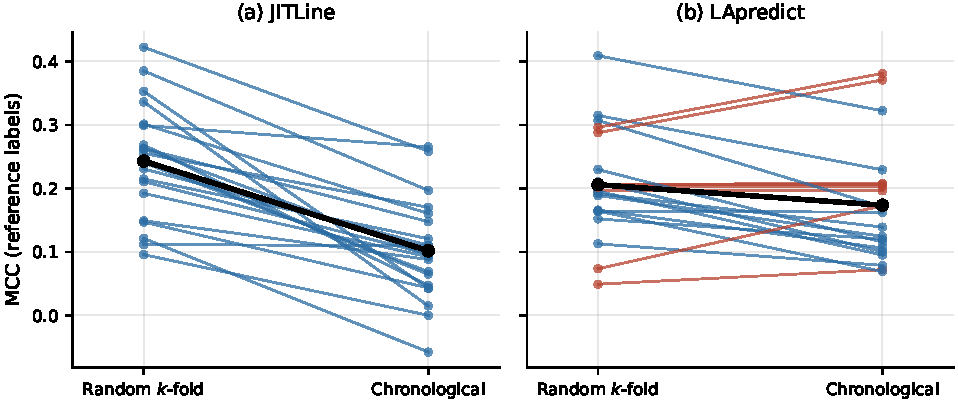
\includegraphics[width=0.92\linewidth]{fig_leakage}
\caption{MCC of each project under random $k$-fold cross-validation and
under the chronological split, for models trained on the reference labels.
The thick line shows the mean.}
\label{fig:leakage}
\end{figure}

The explanation is that in random cross-validation the model is trained on
commits that lie close in time to the test commits, both before and after
them. Commits that are close in time tend to be similar, because they
concern the same parts of the code and are made by the same developers. A
random forest can make use of this similarity. A logistic regression with a
single feature has almost no capacity to do so. The overestimation caused by
random cross-validation therefore increases with the capacity of the model.
A consequence is that a comparison of a simple and a complex model under
random cross-validation favours the complex model. In the present data the
order of the two models is reversed when the evaluation respects time.

\subsection{Effect of scoring against the training labels}

The second effect is the difference between scoring a model against its own
training labels and scoring it against the reference labels.
Table~\ref{tab:selfscore} gives the comparison for the two batch models in
both evaluation settings, and Figure~\ref{fig:selfscore} shows the mean
differences.

\begin{table}[htbp]
\centering\footnotesize
\setlength{\tabcolsep}{3.5pt}
\caption{Self-scored MCC compared with reference-scored MCC for the batch
models. ``Projects'' is the number of projects in which the self-scored value
is higher. The other columns are as in Table~\ref{tab:regime}.}
\label{tab:selfscore}
\resizebox{\linewidth}{!}{%
\begin{tabular}{@{}llcccccccc@{}}
\toprule
Model & Labels & Self & Ref. & HL & 95\% CI & $r$ & Projects & $p$ (family) & $p$ (global) \\
\midrule
\multicolumn{10}{@{}l}{\emph{Random $k$-fold cross-validation}} \\
JITLine & B-SZZ & 0.413 & 0.175 & +0.230 & [+0.189, +0.278] & +0.991 & 20/21 & $<$0.001 & $<$0.001 \\
 & AG-SZZ & 0.304 & 0.116 & +0.180 & [+0.120, +0.246] & +1.000 & 21/21 & $<$0.001 & $<$0.001 \\
 & MA-SZZ & 0.330 & 0.127 & +0.198 & [+0.139, +0.265] & +1.000 & 21/21 & $<$0.001 & $<$0.001 \\
 & L-SZZ & 0.243 & 0.139 & +0.108 & [+0.070, +0.139] & +0.939 & 18/21 & $<$0.001 & 0.001 \\
 & R-SZZ & 0.180 & 0.113 & +0.065 & [+0.030, +0.100] & +0.758 & 17/21 & 0.037 & 0.073 \\
 & RA-SZZ & 0.307 & 0.116 & +0.186 & [+0.122, +0.252] & +1.000 & 21/21 & $<$0.001 & $<$0.001 \\
LApredict & B-SZZ & 0.351 & 0.194 & +0.155 & [+0.121, +0.203] & +0.957 & 20/21 & $<$0.001 & $<$0.001 \\
 & AG-SZZ & 0.247 & 0.200 & +0.051 & [$-$0.012, +0.110] & +0.351 & 12/21 & 0.943 & 1.000 \\
 & MA-SZZ & 0.263 & 0.199 & +0.069 & [+0.006, +0.119] & +0.498 & 13/21 & 0.644 & 1.000 \\
 & L-SZZ & 0.268 & 0.208 & +0.062 & [+0.008, +0.116] & +0.541 & 14/21 & 0.522 & 0.899 \\
 & R-SZZ & 0.178 & 0.202 & $-$0.024 & [$-$0.066, +0.026] & $-$0.221 & 9/21 & 0.971 & 1.000 \\
 & RA-SZZ & 0.260 & 0.200 & +0.060 & [+0.007, +0.117] & +0.481 & 15/21 & 0.711 & 1.000 \\
\midrule
\multicolumn{10}{@{}l}{\emph{Chronological split}} \\
JITLine & B-SZZ & 0.223 & 0.132 & +0.098 & [+0.051, +0.141] & +0.758 & 17/21 & 0.037 & 0.073 \\
 & AG-SZZ & 0.135 & 0.090 & +0.041 & [$-$0.004, +0.088] & +0.420 & 13/21 & 0.766 & 1.000 \\
 & MA-SZZ & 0.140 & 0.079 & +0.054 & [+0.011, +0.097] & +0.628 & 15/21 & 0.233 & 0.415 \\
 & L-SZZ & 0.148 & 0.080 & +0.086 & [+0.045, +0.113] & +0.628 & 18/21 & 0.233 & 0.415 \\
 & R-SZZ & 0.092 & 0.063 & +0.034 & [$-$0.005, +0.073] & +0.403 & 15/21 & 0.777 & 1.000 \\
 & RA-SZZ & 0.140 & 0.086 & +0.052 & [+0.007, +0.100] & +0.524 & 14/21 & 0.561 & 1.000 \\
LApredict & B-SZZ & 0.292 & 0.163 & +0.137 & [+0.104, +0.181] & +0.905 & 20/21 & 0.002 & 0.003 \\
 & AG-SZZ & 0.197 & 0.168 & +0.036 & [$-$0.032, +0.101] & +0.255 & 14/21 & 0.971 & 1.000 \\
 & MA-SZZ & 0.200 & 0.166 & +0.035 & [$-$0.012, +0.098] & +0.299 & 13/21 & 0.971 & 1.000 \\
 & L-SZZ & 0.217 & 0.171 & +0.064 & [$-$0.016, +0.110] & +0.446 & 16/21 & 0.760 & 1.000 \\
 & R-SZZ & 0.167 & 0.173 & +0.006 & [$-$0.056, +0.040] & +0.082 & 11/21 & 0.971 & 1.000 \\
 & RA-SZZ & 0.214 & 0.168 & +0.065 & [$-$0.007, +0.117] & +0.446 & 17/21 & 0.760 & 1.000 \\
\bottomrule
\end{tabular}}
\end{table}

\begin{figure}[htbp]
\centering
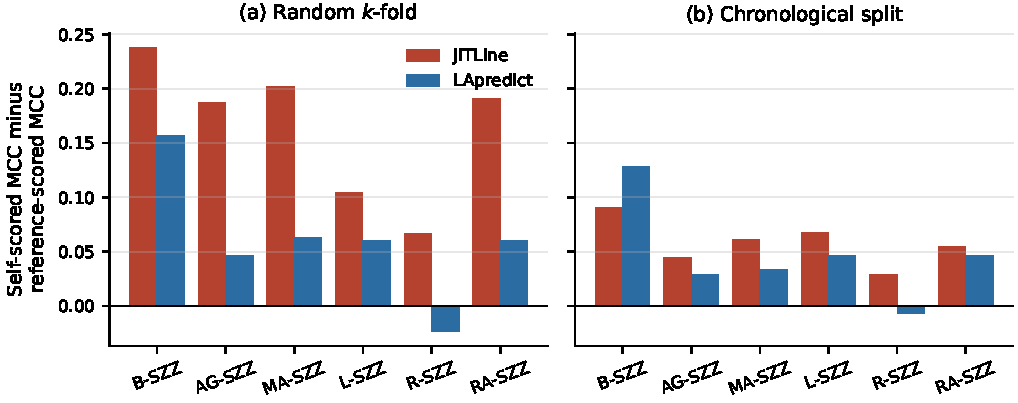
\includegraphics[width=\linewidth]{fig_self_scoring}
\caption{Difference between the self-scored and the reference-scored MCC for
each SZZ variant and both batch models.}
\label{fig:selfscore}
\end{figure}

The largest difference in the whole study is found for JITLine trained on
B-SZZ labels under random cross-validation. The self-scored MCC is 0.413 and
the reference-scored MCC is 0.175. The Hodges--Lehmann estimate of the
difference is 0.230 (95\% CI $[+0.189, +0.278]$), and the self-scored value
is higher in 20 of the 21 projects. A reader who sees only the self-scored
value would conclude that the model is more than twice as good as it is with
respect to the reference.

Under random cross-validation the difference is significant for JITLine with
five of the six variants after the global correction, and for AG-SZZ, MA-SZZ
and RA-SZZ it is positive in all 21 projects. For LApredict it is significant
only with B-SZZ. With R-SZZ the difference for LApredict is even slightly
negative.

Under the chronological split the differences are smaller. For JITLine with
B-SZZ the estimate is 0.098, which is significant within its family but not
after the global correction ($p = 0.073$). For LApredict with B-SZZ it is
0.137 and significant. For ORB, the difference in the chronological-online
setting with B-SZZ is 0.082 (95\% CI $[+0.054, +0.115]$, corrected
$p = 0.004$), and in the prequential setting with the time-averaged summary
it is 0.053 for B-SZZ, 0.042 for MA-SZZ and 0.036 for RA-SZZ, all of which
are significant after the global correction.

Two patterns can be seen in these results. The difference is largest for
B-SZZ, the variant with the highest false-alarm rate, and smallest for R-SZZ
and L-SZZ, which have low false-alarm rates. And for the refined variants it
is much larger for the random forest than for the logistic regression. Both
patterns are consistent with the following explanation. The false positives
of SZZ are not distributed at random over the commits. They are commits whose
lines were later touched by a bug-fixing commit, which is more likely for
large changes and for frequently modified files. A model can learn to
recognise such commits. When it is scored against the SZZ labels, it is
rewarded for this, although these commits are clean according to the
reference. A model with high capacity can learn these regularities better
than a model with a single feature. The case of B-SZZ with LApredict fits
this as well, since the single feature of LApredict is the size of the
change.

This explanation was tested directly with the analysis described in
Section~\ref{sec:additional-method}. A random forest was trained to
distinguish the false positives of B-SZZ from its true positives, using only
the commits flagged by B-SZZ. The mean AUC over the projects is 0.599. With
randomly permuted training labels it is 0.514. The difference is significant
(Hodges--Lehmann estimate $+0.088$, 95\% CI $[+0.041, +0.131]$, higher in 17
of 21 projects, $p = 0.002$). The false positives of B-SZZ can therefore be
distinguished from its true positives better than by chance, which confirms
that the errors of SZZ have a structure that a model can learn. The AUC of
0.60 is modest, however, so this structure is not strong, and it probably
does not account for the whole difference between the two ways of scoring.

\subsection{Effect of the label source in the online setting}\label{sec:label-source}

The third effect is the one for which the study was designed: the loss in
performance when a model is trained on SZZ labels instead of the reference
labels, measured in the most realistic setting. Table~\ref{tab:source}
compares ORB trained on the reference labels with ORB trained on each SZZ
variant in the prequential setting with verification latency. All models are
scored against the reference labels.

\begin{table}[htbp]
\centering\footnotesize
\setlength{\tabcolsep}{4pt}
\caption{ORB trained on the reference labels compared with ORB trained on
each SZZ variant, in the prequential setting with verification latency. HL is
the estimate of the difference (reference minus variant). ``Projects'' is the
number of projects in which the reference-trained model is better.}
\label{tab:source}
\begin{tabular}{@{}lccccccc@{}}
\toprule
Training labels & MCC & HL & 95\% CI & $r$ & Projects & $p$ (family) & $p$ (global) \\
\midrule
\multicolumn{8}{@{}l}{\emph{Time-averaged MCC (reference-trained model: 0.097)}} \\
B-SZZ & 0.058 & +0.041 & [+0.022, +0.052] & +0.879 & 18/21 & $<$0.001 & 0.006 \\
AG-SZZ & 0.036 & +0.060 & [+0.029, +0.085] & +0.818 & 17/21 & $<$0.001 & 0.024 \\
MA-SZZ & 0.035 & +0.064 & [+0.039, +0.085] & +0.896 & 18/21 & $<$0.001 & 0.004 \\
L-SZZ & 0.058 & +0.034 & [+0.014, +0.055] & +0.723 & 16/21 & 0.002 & 0.124 \\
R-SZZ & 0.032 & +0.060 & [+0.042, +0.082] & +0.948 & 19/21 & $<$0.001 & $<$0.001 \\
RA-SZZ & 0.039 & +0.058 & [+0.036, +0.081] & +0.879 & 18/21 & $<$0.001 & 0.006 \\
\midrule
\multicolumn{8}{@{}l}{\emph{Terminal MCC (reference-trained model: 0.069)}} \\
B-SZZ & 0.057 & +0.015 & [$-$0.023, +0.052] & +0.177 & 13/21 & 0.495 & 1.000 \\
AG-SZZ & 0.012 & +0.060 & [+0.020, +0.101] & +0.636 & 15/21 & 0.045 & 0.397 \\
MA-SZZ & $-$0.003 & +0.072 & [+0.019, +0.128] & +0.636 & 16/21 & 0.045 & 0.397 \\
L-SZZ & 0.021 & +0.044 & [+0.011, +0.094] & +0.602 & 15/21 & 0.045 & 0.538 \\
R-SZZ & 0.011 & +0.049 & [+0.014, +0.105] & +0.654 & 16/21 & 0.043 & 0.327 \\
RA-SZZ & 0.019 & +0.045 & [+0.015, +0.093] & +0.619 & 17/21 & 0.045 & 0.443 \\
\bottomrule
\end{tabular}
\end{table}

With the time-averaged MCC, which is the primary summary, the model trained
on the reference labels reaches 0.097 and is better than the models trained
on all six variants. The estimated loss is between 0.034 (L-SZZ) and 0.064
(MA-SZZ). All six confidence intervals exclude zero, the reference-trained
model is better in 16 to 19 of the 21 projects, and five of the six
comparisons remain significant after the correction over all tests. The
exception is L-SZZ, which is significant within its family only. In relative
terms, the SZZ-trained models retain between about one third and three fifths
of the MCC of the reference-trained model. Figure~\ref{fig:source} shows the
means and the estimated differences.

\begin{figure}[htbp]
\centering
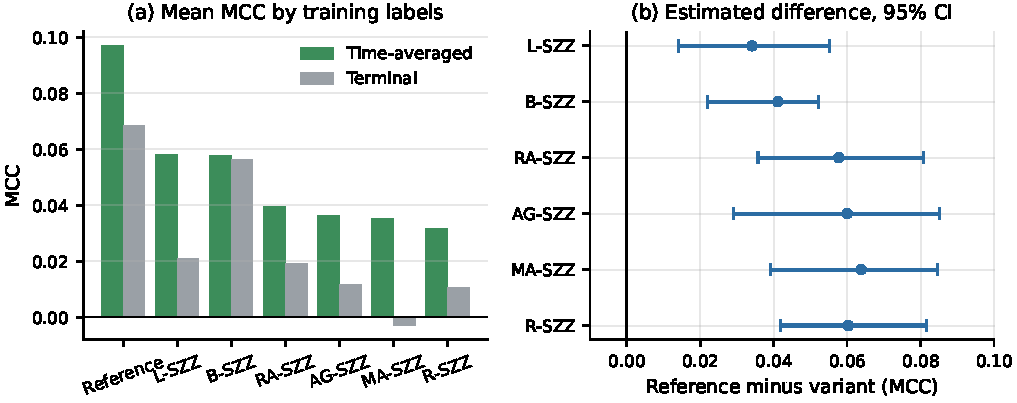
\includegraphics[width=\linewidth]{fig_label_source}
\caption{ORB in the prequential setting with verification latency. (a) Mean
MCC for each source of training labels with both summaries. (b)
Hodges--Lehmann estimate and 95\% confidence interval of the difference
between the reference-trained model and each SZZ-trained model
(time-averaged MCC).}
\label{fig:source}
\end{figure}

The comparison with B-SZZ deserves particular attention. As explained in
Section~\ref{sec:reference}, B-SZZ and the reference labels use the same
blame mechanism and differ in the lines from which the tracing starts. The
loss of 0.041 MCC (95\% CI $[+0.022, +0.052]$) can therefore be read as an
estimate of what the knowledge of the actual bug-fixing lines is worth to an
online learner in this setting.

The size of the loss is not related in a simple way to the recall of the
variants. L-SZZ, with a recall of 0.267, and B-SZZ, with a recall of 0.641,
show almost the same loss, while AG-SZZ, MA-SZZ and RA-SZZ, with recall
values in between, show larger losses. The correlation between the mean loss
and the recall over the six variants is $-0.18$. Which property of the labels
determines the loss cannot be decided from this comparison, because the
variants differ from each other in several respects at the same time. This
question is taken up in the next stage of the thesis.

\paragraph{Results with the terminal MCC.} With the terminal MCC the
reference-trained model is also better than all variants on average, and
five of the six comparisons are significant within the family, although none
remains significant after the global correction. The comparison with B-SZZ is
not significant with this summary ($+0.015$, 95\% CI $[-0.023, +0.052]$).
This is the only comparison in the study for which the two summaries lead to
different conclusions. Figure~\ref{fig:estimators} shows why the terminal
value is less suitable for such comparisons. Its spread over the projects is
almost twice as large as that of the time-averaged value, because it is
computed from the last hundred commits of each project only. The negative
value for MA-SZZ in Table~\ref{tab:mcc-orb} is also a consequence of this
and does not appear with the time-averaged summary.

\begin{figure}[htbp]
\centering
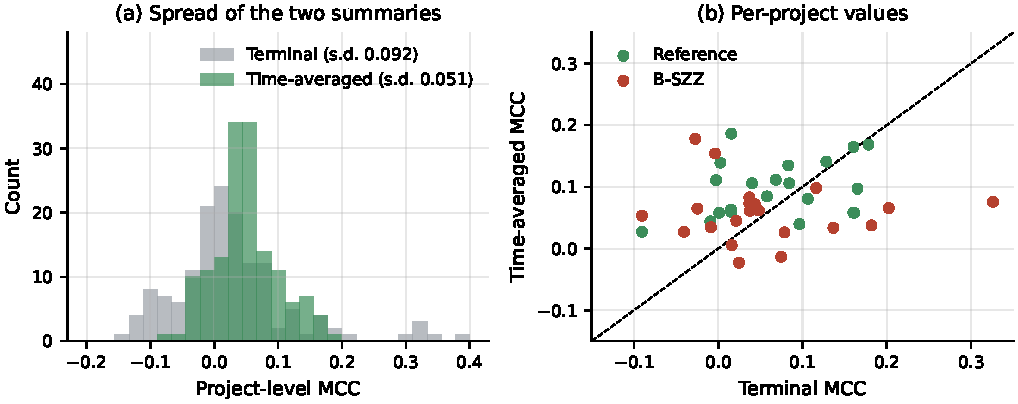
\includegraphics[width=\linewidth]{fig_estimators}
\caption{Comparison of the two summaries of the prequential MCC. (a)
Distribution of the project-level values over all label sources. (b)
Terminal and time-averaged value of each project for models trained on the
reference labels and on B-SZZ labels.}
\label{fig:estimators}
\end{figure}

\paragraph{Check on the availability of arrival times.} For the reference
labels an arrival time is available for only 67.8\% of the defect-introducing
commits, whereas all commits flagged by B-SZZ have one
(Table~\ref{tab:latency-source}). To check whether this difference affects
the comparison, the missing arrival times were imputed from the observed
latency distribution. With imputed arrival times the time-averaged MCC of the
reference-trained model is 0.084 instead of 0.097. It is still higher than
that of the B-SZZ-trained model (0.058). The mean difference is 0.026, the
reference-trained model is better in 16 of 21 projects, and the difference is
significant ($p = 0.010$). With the terminal MCC the difference is 0.004 and
not significant, in line with the result without imputation. The advantage of
the reference labels is thus reduced but not removed when the availability of
arrival times is equalised. The reduction is expected: more than half of the
imputed labels arrive after the waiting period, so the corresponding commits
are first presented to the learner as clean.

\subsection{Combined view of the three effects}

Figure~\ref{fig:ladder} puts the three effects together. It shows the MCC of
six configurations, starting from the one that is closest to common practice
and ending with the most realistic one.

\begin{figure}[htbp]
\centering
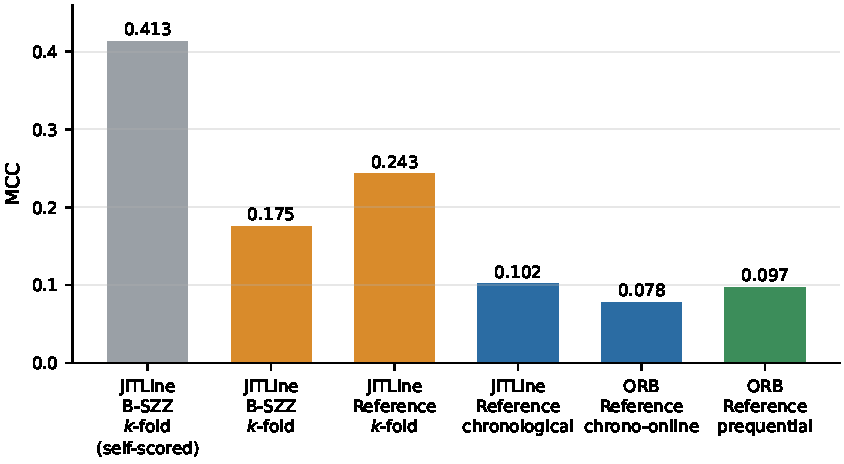
\includegraphics[width=0.9\linewidth]{fig_ladder}
\caption{MCC under increasingly realistic conditions. Each bar is labelled
with the model, the training labels and the evaluation setting. All bars
except the first are scored against the reference labels.}
\label{fig:ladder}
\end{figure}

JITLine trained on B-SZZ labels, evaluated with random cross-validation and
scored against its own labels has an MCC of 0.413. When the same predictions
are scored against the reference labels, the value is 0.175. When the model
is trained on the reference labels and evaluated with the chronological
split, it is 0.102. ORB trained on the reference labels reaches 0.078 in the
chronological-online setting and 0.097 in the prequential setting with
verification latency.

The value that would be reported under common practice is thus about four
times the value obtained under realistic conditions with the best available
labels. Of the three effects, the scoring against the training labels
(0.230) and the random cross-validation (0.137) are several times larger
than the loss caused by training on SZZ labels in the online setting (0.034
to 0.064).

The figure should be read as a description and not as a decomposition. The
bars differ in more than one respect. In particular, the step from the batch
model to the online model changes the learner, the delivery of the labels
and the part of the stream on which the model is tested. This step is
examined next.

\subsection{Label delay and model adaptation}

In Table~\ref{tab:mcc-orb} ORB with reference labels reaches 0.078 in the
chronological-online setting and 0.069 (terminal) or 0.097 (time-averaged)
in the prequential setting. It would be tempting to conclude from these
numbers that verification latency has little effect. Such a conclusion is not
justified, because the two settings differ in three respects: in the
prequential setting the labels are delayed, the model keeps learning, and the
performance is measured over the whole stream with fading instead of over the
second half.

To separate these factors, the experiment with four combinations described in
Section~\ref{sec:additional-method} was carried out.
Table~\ref{tab:factorial} gives the mean MCC of the four cells and the paired
comparisons, and Figure~\ref{fig:factorial} shows the cell means.

\begin{table}[htbp]
\centering\small
\caption{ORB with reference labels in the four combinations of learner
(frozen or adaptive) and label delivery (immediate or delayed). MCC on the
second half of the stream.}
\label{tab:factorial}
\begin{tabular}{@{}lcc@{}}
\toprule
 & Labels immediate & Labels delayed \\
\midrule
Frozen learner & 0.083 & 0.078 \\
Adaptive learner & 0.127 & 0.101 \\
\bottomrule
\end{tabular}

\vspace{0.8em}
\begin{tabular}{@{}lcccc@{}}
\toprule
Comparison & HL & 95\% CI & $r$ & $p$ \\
\midrule
Adaptive minus frozen, labels immediate & +0.042 & [$-$0.002, +0.083] & +0.463 & 0.065 \\
Adaptive minus frozen, labels delayed & +0.015 & [$-$0.011, +0.044] & +0.221 & 0.393 \\
Immediate minus delayed, adaptive learner & +0.023 & [$-$0.011, +0.052] & +0.273 & 0.288 \\
Immediate minus delayed, frozen learner & $-$0.012 & [$-$0.065, +0.047] & $-$0.117 & 0.658 \\
Interaction & $-$0.030 & [$-$0.073, +0.024] & $-$0.247 & 0.338 \\
\bottomrule
\end{tabular}
\end{table}

\begin{figure}[htbp]
\centering
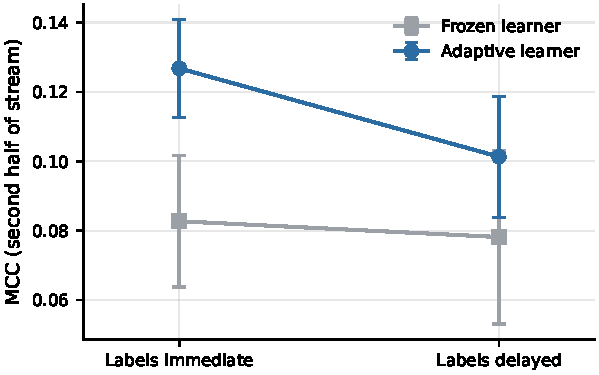
\includegraphics[width=0.6\linewidth]{fig_factorial}
\caption{Mean MCC of the four combinations of learner and label delivery.
The bars show one standard error over the projects.}
\label{fig:factorial}
\end{figure}

The directions of the effects are as expected. An adaptive learner is better
than a frozen one, and delayed labels reduce the performance of the adaptive
learner (0.127 against 0.101). For the frozen learner the delay makes almost
no difference. However, none of the comparisons is statistically significant.
All confidence intervals include zero, including that of the interaction.
With 21 projects, differences of this size, around 0.02 to 0.04 MCC, cannot
be established reliably.

The result is therefore reported as inconclusive. It does not show that
verification latency has no effect. It shows that the effect, if it exists,
is too small to be detected with this design. The experiment also shows that
a design in which several things change at the same time, as in the
comparison of two label sources or two settings, is not suitable for
isolating the effect of latency. In the next stage, experiments are planned
in which the learner and the stream are kept fixed and only the labels are
changed in a controlled way.

\subsection{A case in which B-SZZ labels give a better batch model}

One result in Table~\ref{tab:mcc-batch} is contrary to expectation. In the
chronological setting, JITLine trained on B-SZZ labels has a higher
reference-scored MCC (0.132) than JITLine trained on the reference labels
(0.102). Training on the noisier labels gives the better model.
Figure~\ref{fig:anomaly} shows the difference for each project.

\begin{figure}[htbp]
\centering
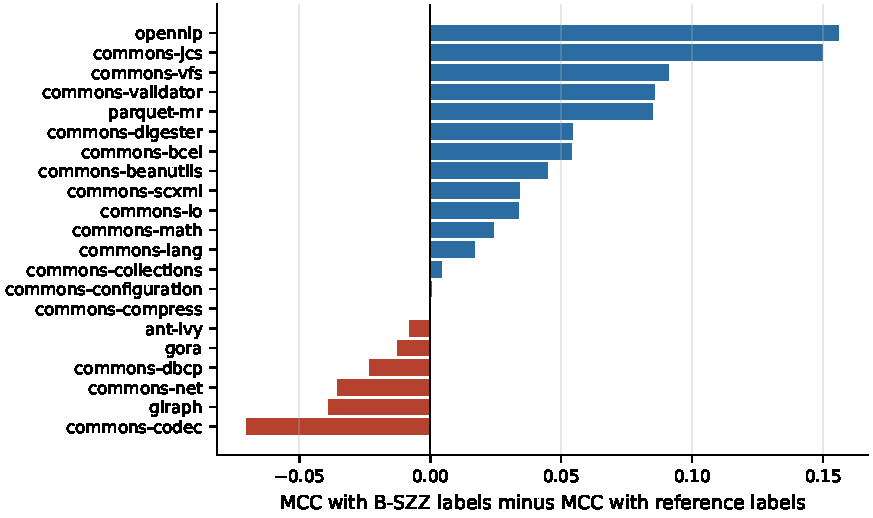
\includegraphics[width=0.78\linewidth]{fig_anomaly}
\caption{Difference between the MCC of JITLine trained on B-SZZ labels and
JITLine trained on the reference labels, for each project (chronological
split, scored against the reference labels).}
\label{fig:anomaly}
\end{figure}

The model trained on B-SZZ labels is better in 15 of the 21 projects. The
differences are stable over the seeds. In 15 projects the mean difference is
more than two standard errors away from zero, and about 95\% of the variance
of the differences between projects is not due to the seeds. The effect was
also present, with a similar size, when other procedures for selecting the
decision threshold of the random forest were tried. It is therefore not a
random fluctuation and not a consequence of the threshold selection.

An obvious hypothesis is that B-SZZ helps because it provides more positive
training examples. The reference labels contain few positive examples in
some projects, and a random forest may learn more from a larger, although
noisier, positive class. To examine this, the difference was correlated with
several characteristics of the projects (Table~\ref{tab:anomaly}).

\begin{table}[htbp]
\centering\small
\caption{Spearman correlation between project characteristics and the
difference shown in Figure~\ref{fig:anomaly}.}
\label{tab:anomaly}
\begin{tabular}{@{}lrr@{}}
\toprule
Project characteristic & Spearman $\rho$ & $p$ \\
\midrule
Defect-introducing commits in the training half & $-$0.249 & 0.28 \\
Defect-introducing commits in total & $-$0.157 & 0.50 \\
Number of commits & $-$0.130 & 0.57 \\
Share of reference labels with an arrival time & $-$0.086 & 0.71 \\
Precision of B-SZZ & $-$0.082 & 0.72 \\
Recall of B-SZZ & $-$0.013 & 0.96 \\
Percentage of commits flagged by B-SZZ & +0.021 & 0.93 \\
Reference defect rate & $-$0.005 & 0.98 \\
B-SZZ flag rate divided by reference defect rate & +0.042 & 0.86 \\
\bottomrule
\end{tabular}
\end{table}

None of the characteristics is significantly correlated with the difference.
The correlation with the number of defect-introducing commits in the training
half has the sign that the hypothesis predicts but is weak. There is also a
project that contradicts the hypothesis. In opennlp the difference is the
largest of all projects ($+0.156$), but B-SZZ flags fewer commits there
(6.9\%) than the reference labels (8.4\%), so it cannot help by providing
more positive examples.

The effect is limited to the batch model. For ORB in the prequential setting
the reference-trained model is better than the B-SZZ-trained model in 18 of
21 projects (Table~\ref{tab:source}). The observation is reported here
because it is stable and may be of interest for further study. Its cause has
not been established, and no explanation is claimed.

\subsection{Robustness checks}\label{sec:robustness}

\paragraph{Fading factor and warm-up period.} The comparison of the label
sources in the prequential setting was repeated for five fading factors and
four lengths of an excluded warm-up period, giving 20 settings for each of
the six variants. Figure~\ref{fig:sensitivity} shows the estimated
differences. In all 120 comparisons the reference-trained model is better,
the confidence interval excludes zero, and the comparison remains
significant after a Holm correction over the 120 comparisons. The estimated
loss for B-SZZ lies between 0.027 and 0.044 over the 20 settings, and the MCC
of the reference-trained model lies between 0.090 and 0.114. The conclusion
of Section~\ref{sec:label-source} does therefore not depend on the choice of
the fading factor or on whether the beginning of the stream is included.
These 120 comparisons are a check of one result under different settings and
should not be counted as separate findings.

\begin{figure}[htbp]
\centering
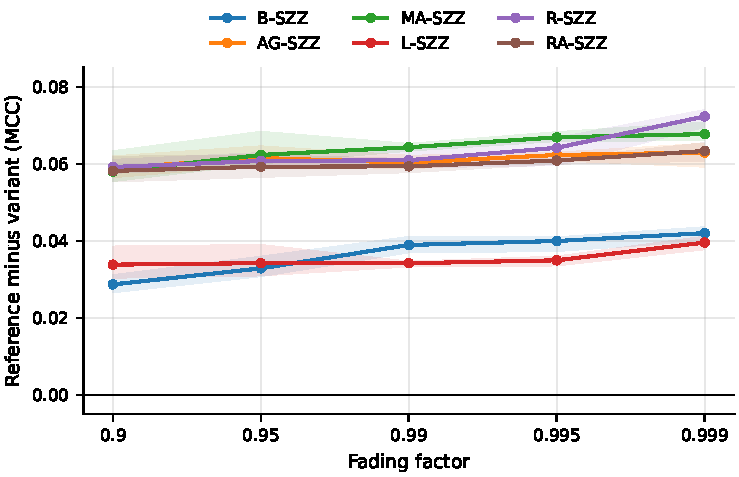
\includegraphics[width=0.8\linewidth]{fig_sensitivity}
\caption{Estimated difference between the reference-trained and the
SZZ-trained model for different fading factors. The lines show the mean over
the four warm-up settings and the shaded bands show their range.}
\label{fig:sensitivity}
\end{figure}

\paragraph{Exclusion of small projects.} All means in this chapter give the
same weight to every project, although the projects differ greatly in size.
Eight projects have fewer than 25 defect-introducing commits in the second
half of their history. Table~\ref{tab:floor} repeats the main comparisons
without these projects. The estimates of the three main effects change by at
most 0.002, and all three remain significant. One result is weaker without
the small projects: the difference between self-scored and reference-scored
MCC for JITLine with B-SZZ in the chronological setting decreases from 0.098
to 0.075 and is no longer significant.

\begin{table}[htbp]
\centering\small
\caption{Main comparisons for all projects and for the 13 projects with at
least 25 defect-introducing commits in the second half of their history.}
\label{tab:floor}
\begin{tabularx}{\linewidth}{@{}>{\raggedright\arraybackslash}Xcc@{}}
\toprule
Comparison & All 21 projects & 13 projects \\
\midrule
Random $k$-fold against chronological split (JITLine, reference labels) &
+0.137 [+0.105, +0.172] & +0.136 [+0.095, +0.171] \\
Self-scored against reference-scored (JITLine, B-SZZ, $k$-fold) &
+0.230 [+0.189, +0.278] & +0.232 [+0.156, +0.322] \\
Self-scored against reference-scored (JITLine, B-SZZ, chronological) &
+0.098 [+0.051, +0.141] & +0.075 [+0.002, +0.135] \\
Reference against B-SZZ training labels (ORB, prequential) &
+0.041 [+0.022, +0.052] & +0.043 [+0.021, +0.067] \\
\bottomrule
\end{tabularx}
\end{table}

\subsection{Discussion and answer to RQ2}

RQ2 asked how the choice of the label source affects the measured
performance of JIT-SDP models under different evaluation settings.

The label source has a clear effect when the models are evaluated
realistically. An online learner trained on the labels of any of the six SZZ
variants performs worse, with respect to the reference labels, than the same
learner trained on the reference labels. The loss is between 0.034 and 0.064
MCC. Since the reference-trained model itself reaches only 0.097, this is a
substantial part of the performance that can be achieved.

The evaluation procedure has a larger effect on the measured performance
than the label source. Random cross-validation increases the MCC of the
random forest model by 0.137, and scoring against the training labels
increases it by up to 0.230. Both effects are larger for the model with
higher capacity. Under these two conditions the differences between label
sources and between models can be hidden or even reversed. For example,
under random cross-validation JITLine appears better than LApredict, and
under the chronological split LApredict is clearly better.

The two issues are connected. Scoring against the training labels is done in
practice because no other labels are available, and this is so because the
labels are produced by a heuristic. The weakness of the labels thus leads to
a weakness of the evaluation. A reference label set that is kept apart from
training, as used in this work, makes the size of this effect visible.

Some limits of these conclusions should be stated. The absolute performance
of all models is low, so the results say little about how useful JIT-SDP
would be with better labels. The results do not show which property of the
SZZ labels causes the loss in the online setting. And the experiment on label
delay and model adaptation remained inconclusive. These points define the
work of the next stage.

\section{Summary of Findings}\label{sec:res-summary}

Table~\ref{tab:findings} summarises the main findings of the first stage
together with the evidence for each.

\begin{table}[htbp]
\centering\small
\caption{Summary of the main findings.}
\label{tab:findings}
\begin{tabularx}{\linewidth}{@{}r>{\raggedright\arraybackslash}X>{\raggedright\arraybackslash}X@{}}
\toprule
 & Finding & Evidence \\
\midrule
1 & The labels of all six SZZ variants differ strongly from the reference
labels. & Precision 0.183 to 0.272; recall 0.267 to 0.641; $\kappa$ with the
reference 0.158 to 0.202 \\
2 & The noise is class-conditional and depends on the variant. & $\rhoz$ from
0.067 to 0.263; $\rhoo$ from 0.359 to 0.733 \\
3 & The variants agree with each other far more than with the reference. &
$\kappa$ between variants 0.33 to 0.93 \\
4 & A large part of the false negatives of the refined variants is caused by
their own filtering. & 30\% to 60\% of the true positives of B-SZZ are
removed \\
5 & Random cross-validation overestimates the performance, more so for the
complex model. & JITLine $+0.137$ MCC in 21 of 21 projects; LApredict
$+0.034$, not significant \\
6 & Scoring against the training labels overestimates the performance
further. & Up to $+0.230$ MCC for JITLine with B-SZZ; the errors of B-SZZ are
learnable (AUC 0.60 against 0.51) \\
7 & In the online setting with verification latency, training on SZZ labels
reduces the performance. & Loss of 0.034 to 0.064 MCC; significant for five
of six variants after global correction \\
8 & The effect of label delay could not be separated reliably with 21
projects. & All comparisons of the four-cell experiment not significant \\
\bottomrule
\end{tabularx}
\end{table}

% ============================================================================
\chapter{Conclusion and Future Work}\label{ch:conclusion}
% ============================================================================

This chapter concludes the report. It summarises the work of the first stage
and its conclusions, discusses the threats to the validity of the results and
describes the work planned for the next stage of the thesis.

\section{Conclusions}

The thesis deals with the effect of the label noise introduced by the SZZ
algorithm on just-in-time software defect prediction. In the first stage,
two studies were carried out on the JIT-Defects4J dataset, which contains
27,319 commits from 21 Apache Java projects and provides reference labels
derived from manually validated bug-fixing lines.

In the first study, the labels of six SZZ variants were generated for all
projects and compared with the reference labels. The comparison showed that
the labels of all variants differ considerably from the reference labels.
The precision of the variants is between 18.3\% and 27.2\%, and their recall
is between 26.7\% and 64.1\%. The errors are of two types whose proportions
depend on the variant. The original algorithm, B-SZZ, flags many clean
commits, whereas the variants that keep only one candidate commit, L-SZZ and
R-SZZ, miss about 70\% of the defect-introducing commits. The refined
variants reduce the false positives of B-SZZ, but a considerable part of
their false negatives is caused by their own filtering rules. The variants
agree with each other much more than with the reference labels, which shows
that agreement between SZZ variants is not a sign of correct labels.

In the second study, three prediction models were trained on the reference
labels and on the labels of each variant and were evaluated in four settings.
The study led to three main results. First, random $k$-fold cross-validation
overestimates the performance compared with a chronological split. For the
random forest model the overestimation is 0.137 MCC and occurs in all 21
projects, while for the logistic regression model with a single feature it is
small. Second, scoring a model against its own SZZ training labels
overestimates the performance further, by up to 0.230 MCC. An additional
analysis showed that the errors of B-SZZ can be predicted from the change
metrics better than by chance, which explains why a model with high capacity
benefits from this way of scoring. Third, when an online learner is evaluated
on the commit stream with verification latency and is scored against the
reference labels, training on the labels of any SZZ variant gives a lower
performance than training on the reference labels. The loss is between 0.034
and 0.064 MCC, compared with an MCC of 0.097 for the model trained on the
reference labels.

Taken together, the results show that the performance values obtained with
the common experimental procedure are much higher than the values obtained
under realistic conditions. In the present data, the first is about four
times the second. The larger part of this difference is due to the evaluation
procedure and a smaller part to the label noise. The label noise nevertheless
causes a loss that is large in relation to the performance that an online
learner can actually achieve.

The research questions RQ1 and RQ2 have thus been answered, and objectives 1
to 4 of Chapter~\ref{ch:gaps} have been achieved.

\section{Threats to Validity}\label{sec:threats}

\subsection{Construct validity}

The most important threat concerns the reference labels. They were obtained
by applying blame to manually validated bug-fixing lines and are not a manual
judgement about each commit. Errors of the blame step are shared by the
reference labels and the SZZ labels and are not detected. The measured noise
is therefore a lower bound. In addition, the set of bug-fixing commits given
to the SZZ variants was taken from the FIX metric of the dataset and may not
be identical to the set from which the reference labels were derived. A part
of the disagreement between SZZ and the reference, in particular a part of
the false negatives of B-SZZ, may be due to this difference and not to the
algorithm.

A second threat concerns the arrival times of the labels. The dataset does
not provide the link between a defect-introducing commit and its fix, so the
arrival times of the reference labels were taken from the SZZ mappings. For
32.2\% of the reference defect-introducing commits no arrival time is
available. The check with imputed arrival times
(Section~\ref{sec:label-source}) shows that the incomplete coverage does not
explain the advantage of the reference labels, but the arrival times that are
available may themselves contain errors. All results of the prequential
setting are affected by this.

A third point is the summary of the prequential MCC. Neither the terminal
nor the time-averaged value is an established standard for MCC. Both were
reported, and the conclusions were checked for different fading factors.

\subsection{Internal validity}

The models used are implementations made or configured for this work. The
random forest model follows the design of JITLine but uses only the change
metrics, and the ORB implementation uses logistic regression base learners.
Other implementations might give different absolute values. The comparisons
in this work are made between conditions that use the same implementation,
so they are less affected by this than the absolute values.

The hyperparameters of the models were not tuned for each label source. This
avoids giving an advantage to one of the label sources, but it also means
that the results hold for the chosen settings.

To reduce the risk of errors in the data processing, the consistency of the
labels used for training with the labels analysed in the first study is
checked automatically before the experiments are run.

\subsection{External validity}

The study uses 21 projects that are all written in Java and belong to the
Apache Software Foundation, sixteen of them to the Apache Commons family.
The results may not hold for projects in other languages, for industrial
projects or for much larger projects. The restriction to this dataset is due
to the need for reference labels at the level of commits, which are not
available for other JIT-SDP datasets. The dataset excludes changes that only
delete code, so defects introduced in this way are not covered. Only the
fourteen change metrics were used as features. Models that use the content of
the changes may be affected by label noise differently.

\subsection{Conclusion validity}

The statistical unit is the project, and there are 21 projects. Differences
below about 0.04 MCC cannot be detected reliably with this number, as the
experiment on label delay showed. Non-significant results in this report
should therefore not be read as evidence that there is no effect.

The analysis was exploratory. The comparisons and their grouping into
families were decided while the results were examined. To account for this,
the correction for multiple comparisons was applied over all 74 tests, and
the main conclusions rest on the results that remain significant after this
correction. All means are unweighted over the projects, which differ in
size. The check without the small projects showed that the main results do
not depend on them.

\section{Future Work}\label{sec:future}

The first stage has shown that SZZ labels reduce the performance of an online
learner, but it has not shown why. The next stage of the thesis addresses
RQ3 and RQ4.

\subsection{Mechanism of the noise effect}

The comparison of label sources cannot identify the cause of the loss,
because two label sources differ in the number of false positives, in the
number of false negatives and in the arrival times of the labels at the same
time. Experiments are therefore planned in which only one property of the
labels is changed at a time.

Two kinds of experiments are planned. In the first, label noise will be
injected into the reference labels in a controlled way. The noise rates will
be chosen according to the pairs $(\rhoz,\rhoo)$ measured in this report, so
that noise with mainly false positives, as in B-SZZ, and noise with mainly
false negatives, as in L-SZZ, can be compared at different levels. In the
second, the B-SZZ labels will be corrected with the help of the reference
labels, once by removing only the false positives and once by restoring only
the false negatives. The change in performance will show which type of error
is responsible for the loss.

The results of the first stage indicate three precautions for these
experiments. Since B-SZZ produces about eight false positives for every false
negative, a comparison in which the same number of labels of each type is
corrected should be included, so that the effect of the type of error is not
confused with the effect of its amount. Since restored defect labels have no
arrival time, a condition in which they are delivered without delay is
needed. And to judge the role of verification latency, a condition in which
all labels are delivered immediately should be included. In addition, the
resampling rate of ORB will be recorded during the experiments, to examine
whether the oversampling of wrongly labelled positive examples
(Section~\ref{sec:models}) contributes to the loss.

\subsection{Reducing the effect of the noise}

Depending on the outcome of these experiments, a modification of the online
learner will be designed that makes it less sensitive to the type of error
that is found to be harmful. The modification must work without access to
clean labels, since these are not available in practice. Two requirements
will be set for it. It should improve the performance when the learner is
trained on SZZ labels, and it should not reduce the performance when the
labels are clean, because a user does not know in advance how noisy the
labels are. The hypotheses, the comparisons and the criteria for accepting
the method will be fixed before the experiments are run, so that the
evaluation of the method is confirmatory and not exploratory.

\subsection{Further directions}

Some further extensions are possible if time permits. The analysis could be
repeated with effort-aware performance measures, which take the cost of
inspecting a commit into account. Other online learners could be included.
The label quality analysis could be extended to other projects if suitable
reference labels become available.

% ------------------------------------------------------------- references
{\small\singlespacing
\begin{thebibliography}{99}
\addcontentsline{toc}{chapter}{References}
\setlength{\itemsep}{1pt}

\bibitem{hall2012slr}
T.~Hall, S.~Beecham, D.~Bowes, D.~Gray, and S.~Counsell, ``A systematic
literature review on fault prediction performance in software engineering,''
\emph{IEEE Transactions on Software Engineering}, vol.~38, no.~6,
pp.~1276--1304, 2012.

\bibitem{rathore2019study}
S.~S. Rathore and S.~Kumar, ``A study on software fault prediction
techniques,'' \emph{Artificial Intelligence Review}, vol.~51, no.~2,
pp.~255--327, 2019.

\bibitem{kamei2013jit}
Y.~Kamei, E.~Shihab, B.~Adams, A.~E. Hassan, A.~Mockus, A.~Sinha, and
N.~Ubayashi, ``A large-scale empirical study of just-in-time quality
assurance,'' \emph{IEEE Transactions on Software Engineering}, vol.~39, no.~6,
pp.~757--773, 2013.

\bibitem{mockus2000risk}
A.~Mockus and D.~M. Weiss, ``Predicting risk of software changes,'' \emph{Bell
Labs Technical Journal}, vol.~5, no.~2, pp.~169--180, 2000.

\bibitem{kim2008classifying}
S.~Kim, E.~J. Whitehead, Jr., and Y.~Zhang, ``Classifying software changes:
Clean or buggy?'' \emph{IEEE Transactions on Software Engineering}, vol.~34,
no.~2, pp.~181--196, 2008.

\bibitem{sliwerski2005szz}
J.~\'{S}liwerski, T.~Zimmermann, and A.~Zeller, ``When do changes induce
fixes?'' in \emph{Proceedings of the International Workshop on Mining Software
Repositories (MSR)}, 2005, pp.~1--5.

\bibitem{herbold2022tangling}
S.~Herbold, A.~Trautsch, B.~Ledel, \emph{et al.}, ``A fine-grained data set and
analysis of tangling in bug fixing commits,'' \emph{Empirical Software
Engineering}, vol.~27, no.~6, article 125, 2022.

\bibitem{dacosta2017maszz}
D.~A. da~Costa, S.~McIntosh, W.~Shang, U.~Kulesza, R.~Coelho, and A.~E.
Hassan, ``A framework for evaluating the results of the SZZ approach for
identifying bug-introducing changes,'' \emph{IEEE Transactions on Software
Engineering}, vol.~43, no.~7, pp.~641--657, 2017.

\bibitem{rosa2021oracle}
G.~Rosa, L.~Pascarella, S.~Scalabrino, R.~Tufano, G.~Bavota, M.~Lanza, and
R.~Oliveto, ``Evaluating SZZ implementations through a developer-informed
oracle,'' in \emph{Proceedings of the 43rd IEEE/ACM International Conference on
Software Engineering (ICSE)}, 2021.

\bibitem{falessi2020order}
D.~Falessi, J.~Huang, L.~Narayana, J.~F. Thai, and B.~Turhan, ``On the need of
preserving order of data when validating within-project defect classifiers,''
\emph{Empirical Software Engineering}, vol.~25, pp.~4805--4830, 2020.

\bibitem{tan2015online}
M.~Tan, L.~Tan, S.~Dara, and C.~Mayeux, ``Online defect prediction for
imbalanced data,'' in \emph{Proceedings of the 37th International Conference on
Software Engineering (ICSE)}, vol.~2, 2015, pp.~99--108.

\bibitem{cabral2019orb}
G.~G. Cabral, L.~L. Minku, E.~Shihab, and S.~Mujahid, ``Class imbalance
evolution and verification latency in just-in-time software defect
prediction,'' in \emph{Proceedings of the 41st International Conference on
Software Engineering (ICSE)}, 2019, pp.~666--676.

\bibitem{zhao2023survey}
Y.~Zhao, K.~Damevski, and H.~Chen, ``A systematic survey of just-in-time
software defect prediction,'' \emph{ACM Computing Surveys}, vol.~55, no.~10,
pp.~1--35, 2023.

\bibitem{mcintosh2018moving}
S.~McIntosh and Y.~Kamei, ``Are fix-inducing changes a moving target? A
longitudinal case study of just-in-time defect prediction,'' \emph{IEEE
Transactions on Software Engineering}, vol.~44, no.~5, pp.~412--428, 2018.

\bibitem{hoang2019deepjit}
T.~Hoang, H.~K. Dam, Y.~Kamei, D.~Lo, and N.~Ubayashi, ``DeepJIT: An end-to-end
deep learning framework for just-in-time defect prediction,'' in
\emph{Proceedings of the 16th International Conference on Mining Software
Repositories (MSR)}, 2019.

\bibitem{hoang2020cc2vec}
T.~Hoang, H.~J. Kang, D.~Lo, and J.~Lawall, ``CC2Vec: Distributed
representations of code changes,'' in \emph{Proceedings of the 42nd
International Conference on Software Engineering (ICSE)}, 2020.

\bibitem{zeng2021lapredict}
Z.~Zeng, Y.~Zhang, H.~Zhang, and L.~Zhang, ``Deep just-in-time defect
prediction: How far are we?'' in \emph{Proceedings of the 30th ACM SIGSOFT
International Symposium on Software Testing and Analysis (ISSTA)}, 2021.

\bibitem{pornprasit2021jitline}
C.~Pornprasit and C.~Tantithamthavorn, ``JITLine: A simpler, better, faster,
finer-grained just-in-time defect prediction,'' in \emph{Proceedings of the
18th International Conference on Mining Software Repositories (MSR)}, 2021,
pp.~369--379.

\bibitem{yang2016effort}
Y.~Yang, Y.~Zhou, J.~Liu, Y.~Zhao, H.~Lu, L.~Xu, B.~Xu, and H.~Leung,
``Effort-aware just-in-time defect prediction: Simple unsupervised models
could be better than supervised models,'' in \emph{Proceedings of the 24th ACM
SIGSOFT International Symposium on Foundations of Software Engineering (FSE)},
2016, pp.~157--168.

\bibitem{rodriguez2020bugs}
G.~Rodr\'{\i}guez-P\'{e}rez, G.~Robles, A.~Serebrenik, A.~Zaidman, D.~M.
Germ\'{a}n, and J.~M. Gonz\'{a}lez-Barahona, ``How bugs are born: A model to
identify how bugs are introduced in software components,'' \emph{Empirical
Software Engineering}, vol.~25, pp.~1294--1340, 2020.

\bibitem{kim2006agszz}
S.~Kim, T.~Zimmermann, K.~Pan, and E.~J. Whitehead, Jr., ``Automatic
identification of bug-introducing changes,'' in \emph{Proceedings of the 21st
IEEE/ACM International Conference on Automated Software Engineering (ASE)},
2006, pp.~81--90.

\bibitem{davies2014rlszz}
S.~Davies, M.~Roper, and M.~Wood, ``Comparing text-based and dependence-based
approaches for determining the origins of bugs,'' \emph{Journal of Software:
Evolution and Process}, vol.~26, no.~1, pp.~107--139, 2014.

\bibitem{neto2018raszz}
E.~C. Neto, D.~A. da~Costa, and U.~Kulesza, ``The impact of refactoring changes
on the SZZ algorithm: An empirical study,'' in \emph{Proceedings of the 25th
IEEE International Conference on Software Analysis, Evolution and
Reengineering (SANER)}, 2018, pp.~380--390.

\bibitem{rodriguez2018szz}
G.~Rodr\'{\i}guez-P\'{e}rez, G.~Robles, and J.~M. Gonz\'{a}lez-Barahona,
``Reproducibility and credibility in empirical software engineering: A case
study based on a systematic literature review of the use of the SZZ
algorithm,'' \emph{Information and Software Technology}, vol.~99,
pp.~164--176, 2018.

\bibitem{rosa2023szzvariants}
G.~Rosa, L.~Pascarella, S.~Scalabrino, R.~Tufano, G.~Bavota, M.~Lanza, and
R.~Oliveto, ``A comprehensive evaluation of SZZ variants through a
developer-informed oracle,'' \emph{Journal of Systems and Software}, vol.~202,
article 111729, 2023.

\bibitem{herzig2013tangled}
K.~Herzig and A.~Zeller, ``The impact of tangled code changes,'' in
\emph{Proceedings of the 10th Working Conference on Mining Software
Repositories (MSR)}, 2013, pp.~121--130.

\bibitem{kim2011noise}
S.~Kim, H.~Zhang, R.~Wu, and L.~Gong, ``Dealing with noise in defect
prediction,'' in \emph{Proceedings of the 33rd International Conference on
Software Engineering (ICSE)}, 2011, pp.~481--490.

\bibitem{tantithamthavorn2015mislabelling}
C.~Tantithamthavorn, S.~McIntosh, A.~E. Hassan, A.~Ihara, and K.~Matsumoto,
``The impact of mislabelling on the performance and interpretation of defect
prediction models,'' in \emph{Proceedings of the 37th International Conference
on Software Engineering (ICSE)}, 2015, pp.~812--823.

\bibitem{fan2021mislabeled}
Y.~Fan, X.~Xia, D.~A. da~Costa, D.~Lo, A.~E. Hassan, and S.~Li, ``The impact of
changes mislabeled by SZZ on just-in-time defect prediction,'' \emph{IEEE
Transactions on Software Engineering}, vol.~47, no.~8, pp.~1559--1586, 2021.

\bibitem{gama2013prequential}
J.~Gama, R.~Sebasti\~{a}o, and P.~P. Rodrigues, ``On evaluating stream learning
algorithms,'' \emph{Machine Learning}, vol.~90, no.~3, pp.~317--346, 2013.

\bibitem{cabral2023reliable}
G.~G. Cabral and L.~L. Minku, ``Towards reliable online just-in-time software
defect prediction,'' \emph{IEEE Transactions on Software Engineering}, vol.~49,
no.~3, pp.~1342--1358, 2023.

\bibitem{tabassum2020cross}
S.~Tabassum, L.~L. Minku, D.~Feng, G.~G. Cabral, and L.~Song, ``An
investigation of cross-project learning in online just-in-time software defect
prediction,'' in \emph{Proceedings of the 42nd International Conference on
Software Engineering (ICSE)}, 2020, pp.~554--565.

\bibitem{yao2020mcc}
J.~Yao and M.~Shepperd, ``Assessing software defection prediction performance:
Why using the Matthews correlation coefficient matters,'' in \emph{Proceedings
of the 24th International Conference on Evaluation and Assessment in Software
Engineering (EASE)}, 2020, pp.~120--129.

\bibitem{matthews1975mcc}
B.~W. Matthews, ``Comparison of the predicted and observed secondary structure
of T4 phage lysozyme,'' \emph{Biochimica et Biophysica Acta (BBA) -- Protein
Structure}, vol.~405, no.~2, pp.~442--451, 1975.

\bibitem{chicco2020mcc}
D.~Chicco and G.~Jurman, ``The advantages of the Matthews correlation
coefficient (MCC) over F1 score and accuracy in binary classification
evaluation,'' \emph{BMC Genomics}, vol.~21, article 6, 2020.

\bibitem{cohen1960kappa}
J.~Cohen, ``A coefficient of agreement for nominal scales,'' \emph{Educational
and Psychological Measurement}, vol.~20, no.~1, pp.~37--46, 1960.

\bibitem{landis1977kappa}
J.~R. Landis and G.~G. Koch, ``The measurement of observer agreement for
categorical data,'' \emph{Biometrics}, vol.~33, no.~1, pp.~159--174, 1977.

\bibitem{oza2001onlinebagging}
N.~C. Oza and S.~Russell, ``Online bagging and boosting,'' in
\emph{Proceedings of the 8th International Workshop on Artificial Intelligence
and Statistics (AISTATS)}, 2001, pp.~229--236.

\bibitem{wang2015oob}
S.~Wang, L.~L. Minku, and X.~Yao, ``Resampling-based ensemble methods for
online class imbalance learning,'' \emph{IEEE Transactions on Knowledge and
Data Engineering}, vol.~27, no.~5, pp.~1356--1368, 2015.

\bibitem{natarajan2013noisy}
N.~Natarajan, I.~S. Dhillon, P.~Ravikumar, and A.~Tewari, ``Learning with noisy
labels,'' in \emph{Advances in Neural Information Processing Systems (NIPS)},
2013.

\bibitem{han2018coteaching}
B.~Han, Q.~Yao, X.~Yu, G.~Niu, M.~Xu, W.~Hu, I.~Tsang, and M.~Sugiyama,
``Co-teaching: Robust training of deep neural networks with extremely noisy
labels,'' in \emph{Advances in Neural Information Processing Systems
(NeurIPS)}, 2018.

\bibitem{northcutt2021confident}
C.~G. Northcutt, L.~Jiang, and I.~L. Chuang, ``Confident learning: Estimating
uncertainty in dataset labels,'' \emph{Journal of Artificial Intelligence
Research}, vol.~70, pp.~1373--1411, 2021.

\bibitem{keshavarz2022apachejit}
H.~Keshavarz and M.~Nagappan, ``ApacheJIT: A large dataset for just-in-time
defect prediction,'' in \emph{Proceedings of the 19th International Conference
on Mining Software Repositories (MSR)}, 2022.

\bibitem{mahbub2023defectors}
P.~Mahbub, O.~Shuvo, and M.~M. Rahman, ``Defectors: A large, diverse Python
dataset for defect prediction,'' in \emph{Proceedings of the 20th International
Conference on Mining Software Repositories (MSR)}, 2023.

\bibitem{ni2022jitdefects4j}
C.~Ni, W.~Wang, K.~Yang, X.~Xia, K.~Liu, and D.~Lo, ``The best of both worlds:
Integrating semantic features with expert features for defect prediction and
localization,'' in \emph{Proceedings of the 30th ACM Joint European Software
Engineering Conference and Symposium on the Foundations of Software
Engineering (ESEC/FSE)}, 2022, pp.~672--683.

\bibitem{breiman2001rf}
L.~Breiman, ``Random forests,'' \emph{Machine Learning}, vol.~45, no.~1,
pp.~5--32, 2001.

\bibitem{chawla2002smote}
N.~V. Chawla, K.~W. Bowyer, L.~O. Hall, and W.~P. Kegelmeyer, ``SMOTE:
Synthetic minority over-sampling technique,'' \emph{Journal of Artificial
Intelligence Research}, vol.~16, pp.~321--357, 2002.

\bibitem{wilcoxon1945}
F.~Wilcoxon, ``Individual comparisons by ranking methods,'' \emph{Biometrics
Bulletin}, vol.~1, no.~6, pp.~80--83, 1945.

\bibitem{hodges1963}
J.~L. Hodges and E.~L. Lehmann, ``Estimates of location based on rank tests,''
\emph{The Annals of Mathematical Statistics}, vol.~34, no.~2, pp.~598--611,
1963.

\bibitem{efron1979bootstrap}
B.~Efron, ``Bootstrap methods: Another look at the jackknife,'' \emph{The
Annals of Statistics}, vol.~7, no.~1, pp.~1--26, 1979.

\bibitem{holm1979}
S.~Holm, ``A simple sequentially rejective multiple test procedure,''
\emph{Scandinavian Journal of Statistics}, vol.~6, no.~2, pp.~65--70, 1979.

\end{thebibliography}
}

\end{document}
